\providecommand{\Mod}{\mathbb{M}od}
\providecommand{\HomA}{\mathrm{Hom}_{A}}
\providecommand{\HomB}{\mathrm{Hom}_{B}}
\providecommand{\HomC}{\mathrm{Hom}_{C}}
\providecommand{\HomD}{\mathrm{Hom}_{D}}
\providecommand{\HomE}{\mathrm{Hom}_{E}}
\providecommand{\rvbendL}{\tikz[baseline=-0.5ex,x=0.9em,y=0.9em]%
\draw[->] (0.8,0.7) .. controls (-0.6,0.7) and (-0.6,-0.7) .. (0.8,-0.7);}
\providecommand{\rvbendR}{\tikz[baseline=-0.5ex,x=0.9em,y=0.9em]%
\draw[->] (-0.8,-0.7) .. controls (0.6,-0.7) and (0.6,0.7) .. (-0.8,0.7);}

\section{可表示模}\label{sec:representable-modules}

虚拟装备中的任何竖直箭头 $f\colon A\to B$ 都带有一对与之相关联的水平箭头
$B\xrightarrow{\HomB(f,B)}A$ 与 $A\xrightarrow{\HomB(B,f)}B$，它们定义为诸水平
单位箭头的限制，并拥有与通常\trDoubleCategory{}中的\emph{\trCompanion}（companion）与%
\emph{\trConjoint}（conjoint）相类似的\trUniversalProperty{} $[47]$。
在模的\trVirtualEquipment{}中，把它们合情理地称作一个\trFunctor{}作为模的%
\emph{左表示与右表示}（left and right representations of a functor as a module），
并沿用这套熟悉的术语与记号，因为它们恰好与定义 3.5.1 和 7.4.7 中引入的左、右
可表示元完全重合。

\begin{proposition}[可表示元的\trCompanion{}与\trConjoint{}关系]%
\label{prop:representable-restriction-application}
对于模的\trVirtualEquipment{}中的任何\trFunctor{} $f\colon A\to B$，存在%
\trCanonical{}限制胞腔（下左两图所示）与应用胞腔（下右两图所示）
\begin{center}
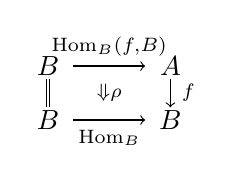
\begin{tikzpicture}[x=1.3em,y=1.3em]
  \node (a1) at (0,1.5)   {$B$};
  \node (a2) at (3.4,1.5) {$A$};
  \node (a3) at (0,0)     {$B$};
  \node (a4) at (3.4,0)   {$B$};
  \draw[->] (0.7,1.5) -- node[above]{$\scriptstyle\HomB(f,B)$} (2.7,1.5);
  \draw[double,double distance=0.6pt] (0,1.15) -- (0,0.35);
  \draw[->] (3.4,1.15) -- (3.4,0.35);
  \node at (3.9,0.75) {$\scriptstyle f$};
  \node at (1.7,0.75) {$\scriptstyle\Downarrow\rho$};
  \draw[->] (0.7,0) -- node[below]{$\scriptstyle\HomB$} (2.7,0);
\end{tikzpicture}
\qquad
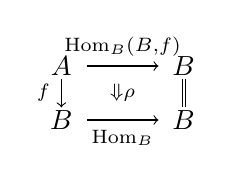
\begin{tikzpicture}[x=1.3em,y=1.3em]
  \node (b1) at (0,1.5)   {$A$};
  \node (b2) at (3.4,1.5) {$B$};
  \node (b3) at (0,0)     {$B$};
  \node (b4) at (3.4,0)   {$B$};
  \draw[->] (0.7,1.5) -- node[above]{$\scriptstyle\HomB(B,f)$} (2.7,1.5);
  \draw[->] (0,1.15) -- (0,0.35);
  \node at (-0.5,0.75) {$\scriptstyle f$};
  \draw[double,double distance=0.6pt] (3.4,1.15) -- (3.4,0.35);
  \node at (1.7,0.75) {$\scriptstyle\Downarrow\rho$};
  \draw[->] (0.7,0) -- node[below]{$\scriptstyle\HomB$} (2.7,0);
\end{tikzpicture}
\qquad
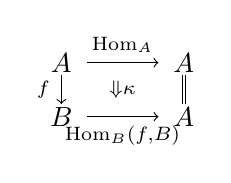
\begin{tikzpicture}[x=1.3em,y=1.3em]
  \node (c1) at (0,1.5)   {$A$};
  \node (c2) at (3.4,1.5) {$A$};
  \node (c3) at (0,0)     {$B$};
  \node (c4) at (3.4,0)   {$A$};
  \draw[->] (0.7,1.5) -- node[above]{$\scriptstyle\HomA$} (2.7,1.5);
  \draw[->] (0,1.15) -- (0,0.35);
  \node at (-0.5,0.75) {$\scriptstyle f$};
  \draw[double,double distance=0.6pt] (3.4,1.15) -- (3.4,0.35);
  \node at (1.7,0.75) {$\scriptstyle\Downarrow\kappa$};
  \draw[->] (0.7,0) -- node[below]{$\scriptstyle\HomB(f,B)$} (2.7,0);
\end{tikzpicture}
\qquad
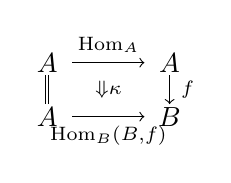
\begin{tikzpicture}[x=1.3em,y=1.3em]
  \node (d1) at (0,1.5)   {$A$};
  \node (d2) at (3.4,1.5) {$A$};
  \node (d3) at (0,0)     {$A$};
  \node (d4) at (3.4,0)   {$B$};
  \draw[->] (0.7,1.5) -- node[above]{$\scriptstyle\HomA$} (2.7,1.5);
  \draw[double,double distance=0.6pt] (0,1.15) -- (0,0.35);
  \draw[->] (3.4,1.15) -- (3.4,0.35);
  \node at (3.9,0.75) {$\scriptstyle f$};
  \node at (1.7,0.75) {$\scriptstyle\Downarrow\kappa$};
  \draw[->] (0.7,0) -- node[below]{$\scriptstyle\HomB(B,f)$} (2.7,0);
\end{tikzpicture}
\end{center}
它们在单位模 $A\xrightarrow{\HomA}A$、$B\xrightarrow{\HomB}B$ 与左、右可表示模
$B\xrightarrow{\HomB(f,B)}A$、$A\xrightarrow{\HomB(B,f)}B$ 之间定义一元映射。
这些胞腔满足如下恒等式\footnote{(8.4.3) 第二行右图之中间行末节点，原书印作
$A$；按其上一行 $\HomB$（$B$ 处之单位模，$B\to B$）之靶当为 $B$，此处径改。
——译者注}：
\begin{rveq}\label{eq:unary-map-identities}
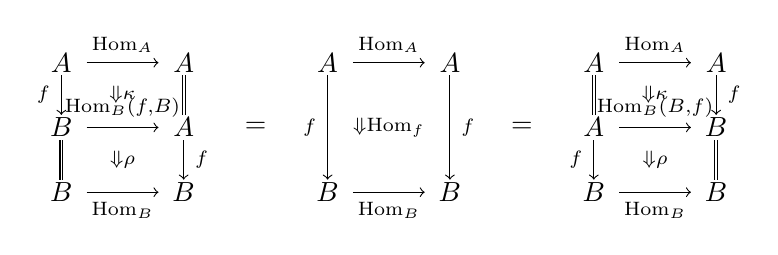
\begin{tikzpicture}[x=1.3em,y=1.3em]
  \node (e1) at (0,3.0)   {$A$};
  \node (e2) at (3.4,3.0) {$A$};
  \node (e3) at (0,1.2)   {$B$};
  \node (e4) at (3.4,1.2) {$A$};
  \node (e5) at (0,-0.6)  {$B$};
  \node (e6) at (3.4,-0.6){$B$};
  \draw[->] (0.7,3.0) -- node[above]{$\scriptstyle\HomA$} (2.7,3.0);
  \draw[->] (0.7,1.2) -- node[above]{$\scriptstyle\HomB(f,B)$} (2.7,1.2);
  \draw[->] (0.7,-0.6) -- node[below]{$\scriptstyle\HomB$} (2.7,-0.6);
  \draw[->] (0,2.65) -- (0,1.55);
  \node at (-0.5,2.1) {$\scriptstyle f$};
  \draw[double,double distance=0.6pt] (3.4,2.65) -- (3.4,1.55);
  \draw[double,double distance=0.6pt] (0,0.85) -- (0,-0.25);
  \draw[->] (3.4,0.85) -- (3.4,-0.25);
  \node at (3.9,0.3) {$\scriptstyle f$};
  \node at (1.7,2.1)  {$\scriptstyle\Downarrow\kappa$};
  \node at (1.7,0.3)  {$\scriptstyle\Downarrow\rho$};
  \node at (5.4,1.2) {$=$};
  \begin{scope}[shift={(7.4,0)}]
  \node (f1) at (0,3.0)   {$A$};
  \node (f2) at (3.4,3.0) {$A$};
  \node (f3) at (0,-0.6)  {$B$};
  \node (f4) at (3.4,-0.6){$B$};
  \draw[->] (0.7,3.0) -- node[above]{$\scriptstyle\HomA$} (2.7,3.0);
  \draw[->] (0.7,-0.6) -- node[below]{$\scriptstyle\HomB$} (2.7,-0.6);
  \draw[->] (0,2.65) -- (0,-0.25);
  \node at (-0.5,1.2) {$\scriptstyle f$};
  \draw[->] (3.4,2.65) -- (3.4,-0.25);
  \node at (3.9,1.2) {$\scriptstyle f$};
  \node at (1.7,1.2) {$\scriptstyle\Downarrow\mathrm{Hom}_{f}$};
  \end{scope}
  \node at (12.8,1.2) {$=$};
  \begin{scope}[shift={(14.8,0)}]
  \node (g1) at (0,3.0)   {$A$};
  \node (g2) at (3.4,3.0) {$A$};
  \node (g3) at (0,1.2)   {$A$};
  \node (g4) at (3.4,1.2) {$B$};
  \node (g5) at (0,-0.6)  {$B$};
  \node (g6) at (3.4,-0.6){$B$};
  \draw[->] (0.7,3.0) -- node[above]{$\scriptstyle\HomA$} (2.7,3.0);
  \draw[->] (0.7,1.2) -- node[above]{$\scriptstyle\HomB(B,f)$} (2.7,1.2);
  \draw[->] (0.7,-0.6) -- node[below]{$\scriptstyle\HomB$} (2.7,-0.6);
  \draw[double,double distance=0.6pt] (0,2.65) -- (0,1.55);
  \draw[->] (3.4,2.65) -- (3.4,1.55);
  \node at (3.9,2.1) {$\scriptstyle f$};
  \draw[->] (0,0.85) -- (0,-0.25);
  \node at (-0.5,0.3) {$\scriptstyle f$};
  \draw[double,double distance=0.6pt] (3.4,0.85) -- (3.4,-0.25);
  \node at (1.7,2.1) {$\scriptstyle\Downarrow\kappa$};
  \node at (1.7,0.3) {$\scriptstyle\Downarrow\rho$};
  \end{scope}
\end{tikzpicture}
\end{rveq}
以及
\begin{rveq}\label{eq:companion-conjoint-relations}
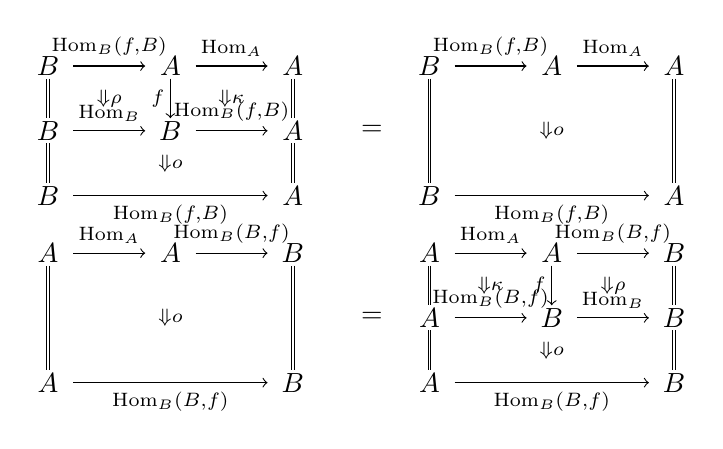
\begin{tikzpicture}[x=1.3em,y=1.3em]
  \node (h1) at (0,2.6)   {$B$};
  \node (h2) at (3.4,2.6) {$A$};
  \node (h3) at (6.8,2.6) {$A$};
  \node (h4) at (0,0.8)   {$B$};
  \node (h5) at (3.4,0.8) {$B$};
  \node (h6) at (6.8,0.8) {$A$};
  \node (h7) at (0,-1.0)  {$B$};
  \node (h8) at (6.8,-1.0){$A$};
  \draw[->] (0.7,2.6) -- node[above]{$\scriptstyle\HomB(f,B)$} (2.7,2.6);
  \draw[->] (4.1,2.6) -- node[above]{$\scriptstyle\HomA$} (6.1,2.6);
  \draw[->] (0.7,0.8) -- node[above]{$\scriptstyle\HomB$} (2.7,0.8);
  \draw[->] (4.1,0.8) -- node[above]{$\scriptstyle\HomB(f,B)$} (6.1,0.8);
  \draw[->] (0.7,-1.0) -- node[below]{$\scriptstyle\HomB(f,B)$} (6.1,-1.0);
  \draw[double,double distance=0.6pt] (0,2.25) -- (0,1.15);
  \draw[->] (3.4,2.25) -- (3.4,1.15);
  \node at (3.05,1.7) {$\scriptstyle f$};
  \draw[double,double distance=0.6pt] (6.8,2.25) -- (6.8,1.15);
  \draw[double,double distance=0.6pt] (0,0.45) -- (0,-0.65);
  \draw[double,double distance=0.6pt] (6.8,0.45) -- (6.8,-0.65);
  \node at (1.7,1.7)  {$\scriptstyle\Downarrow\rho$};
  \node at (5.1,1.7)  {$\scriptstyle\Downarrow\kappa$};
  \node at (3.4,-0.1) {$\scriptstyle\Downarrow o$};
  \node at (9.0,0.8) {$=$};
  \begin{scope}[shift={(10.6,0)}]
  \node (i1) at (0,2.6)   {$B$};
  \node (i2) at (3.4,2.6) {$A$};
  \node (i3) at (6.8,2.6) {$A$};
  \node (i4) at (0,-1.0)  {$B$};
  \node (i5) at (6.8,-1.0){$A$};
  \draw[->] (0.7,2.6) -- node[above]{$\scriptstyle\HomB(f,B)$} (2.7,2.6);
  \draw[->] (4.1,2.6) -- node[above]{$\scriptstyle\HomA$} (6.1,2.6);
  \draw[->] (0.7,-1.0) -- node[below]{$\scriptstyle\HomB(f,B)$} (6.1,-1.0);
  \draw[double,double distance=0.6pt] (0,2.25) -- (0,-0.65);
  \draw[double,double distance=0.6pt] (6.8,2.25) -- (6.8,-0.65);
  \node at (3.4,0.8) {$\scriptstyle\Downarrow o$};
  \end{scope}
  \begin{scope}[shift={(0,-5.2)}]
  \node (j1) at (0,2.6)   {$A$};
  \node (j2) at (3.4,2.6) {$A$};
  \node (j3) at (6.8,2.6) {$B$};
  \node (j4) at (0,-1.0)  {$A$};
  \node (j5) at (6.8,-1.0){$B$};
  \draw[->] (0.7,2.6) -- node[above]{$\scriptstyle\HomA$} (2.7,2.6);
  \draw[->] (4.1,2.6) -- node[above]{$\scriptstyle\HomB(B,f)$} (6.1,2.6);
  \draw[->] (0.7,-1.0) -- node[below]{$\scriptstyle\HomB(B,f)$} (6.1,-1.0);
  \draw[double,double distance=0.6pt] (0,2.25) -- (0,-0.65);
  \draw[double,double distance=0.6pt] (6.8,2.25) -- (6.8,-0.65);
  \node at (3.4,0.8) {$\scriptstyle\Downarrow o$};
  \end{scope}
  \node at (9.0,-4.4) {$=$};
  \begin{scope}[shift={(10.6,-5.2)}]
  \node (k1) at (0,2.6)   {$A$};
  \node (k2) at (3.4,2.6) {$A$};
  \node (k3) at (6.8,2.6) {$B$};
  \node (k4) at (0,0.8)   {$A$};
  \node (k5) at (3.4,0.8) {$B$};
  \node (k6) at (6.8,0.8) {$B$};
  \node (k7) at (0,-1.0)  {$A$};
  \node (k8) at (6.8,-1.0){$B$};
  \draw[->] (0.7,2.6) -- node[above]{$\scriptstyle\HomA$} (2.7,2.6);
  \draw[->] (4.1,2.6) -- node[above]{$\scriptstyle\HomB(B,f)$} (6.1,2.6);
  \draw[->] (0.7,0.8) -- node[above]{$\scriptstyle\HomB(B,f)$} (2.7,0.8);
  \draw[->] (4.1,0.8) -- node[above]{$\scriptstyle\HomB$} (6.1,0.8);
  \draw[->] (0.7,-1.0) -- node[below]{$\scriptstyle\HomB(B,f)$} (6.1,-1.0);
  \draw[double,double distance=0.6pt] (0,2.25) -- (0,1.15);
  \draw[->] (3.4,2.25) -- (3.4,1.15);
  \node at (3.05,1.7) {$\scriptstyle f$};
  \draw[double,double distance=0.6pt] (6.8,2.25) -- (6.8,1.15);
  \draw[double,double distance=0.6pt] (0,0.45) -- (0,-0.65);
  \draw[double,double distance=0.6pt] (6.8,0.45) -- (6.8,-0.65);
  \node at (1.7,1.7)  {$\scriptstyle\Downarrow\kappa$};
  \node at (5.1,1.7)  {$\scriptstyle\Downarrow\rho$};
  \node at (3.4,-0.1) {$\scriptstyle\Downarrow o$};
  \end{scope}
\end{tikzpicture}
\end{rveq}
\end{proposition}

\begin{proof}
诸一元模映射 $\kappa$ 由 \eqref{eq:unary-map-identities} 中的诸等式、通过诉诸
命题 8.2.1 中限制胞腔的\trUniversalProperty{}而定义。
诸关系 \eqref{eq:companion-conjoint-relations} 本也可以经由命题 8.2.4 与引理
8.3.10、8.3.15 从定理 8.2.6 的诸公理直接验证。
为求变化，我们诉诸引理 8.1.16，把\trVirtualEquipment{}中的每个胞腔刻画为%
\trHomotopyTwoCategory{}中的\trNaturalTransformation。

我们对右可表示元证明此事。由注 8.3.13，\eqref{eq:companion-conjoint-relations}
中最右边那个等式之左侧的二元模映射表示为下左图的\trNaturalTransformation，而
右侧的复合则表示为下右图：
\begin{center}
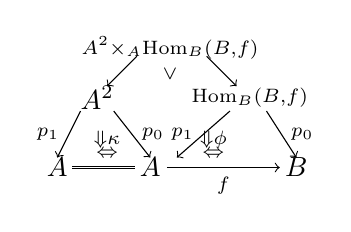
\begin{tikzpicture}[x=1.2em,y=1.2em]
  \node (P) at (3.4,4.6) {$\scriptstyle A^{2}\times_{A}\HomB(B,f)$};
  \node (A2) at (1.2,3.1) {$A^{2}$};
  \node (H)  at (5.8,3.1) {$\scriptstyle\HomB(B,f)$};
  \draw[->] (2.4,4.35) -- (1.5,3.45);
  \draw[->] (4.5,4.35) -- (5.4,3.45);
  \node at (3.4,3.8) {$\scriptstyle\vee$};
  \draw[->] (0.7,2.7) -- node[left,pos=0.5]{$\scriptstyle p_{1}$} (0,1.3);
  \draw[->] (1.7,2.7) -- node[right,pos=0.5]{$\scriptstyle p_{0}$} (2.8,1.3);
  \node at (1.5,1.85) {$\scriptstyle\Downarrow\kappa$};
  \node at (1.5,1.4)  {$\scriptstyle\Leftrightarrow$};
  \draw[->] (5.2,2.7) -- node[left,pos=0.5]{$\scriptstyle p_{1}$} (3.6,1.3);
  \draw[->] (6.3,2.7) -- node[right,pos=0.5]{$\scriptstyle p_{0}$} (7.2,1.3);
  \node at (4.7,1.85) {$\scriptstyle\Downarrow\phi$};
  \node at (4.7,1.4)  {$\scriptstyle\Leftrightarrow$};
  \node (a1) at (0,1.0)   {$A$};
  \node (a2) at (2.8,1.0) {$A$};
  \draw[double,double distance=0.6pt] (0.45,1.0) -- (2.35,1.0);
  \node (b1) at (7.2,1.0) {$B$};
  \draw[->] (3.3,1.0) -- node[below]{$\scriptstyle f$} (6.7,1.0);
\end{tikzpicture}
\qquad $=$ \qquad
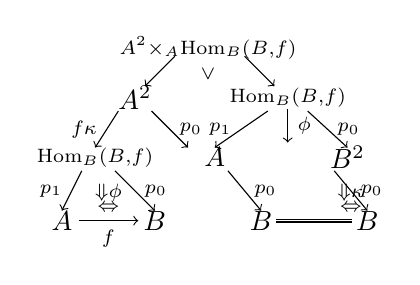
\begin{tikzpicture}[x=1.2em,y=1.2em]
  \node (P) at (4.0,5.2) {$\scriptstyle A^{2}\times_{A}\HomB(B,f)$};
  \node (A2) at (1.8,3.7) {$A^{2}$};
  \node (H)  at (6.4,3.7) {$\scriptstyle\HomB(B,f)$};
  \draw[->] (3.0,4.95) -- (2.1,4.05);
  \draw[->] (5.1,4.95) -- (6.0,4.05);
  \node at (4.0,4.4) {$\scriptstyle\vee$};
  \draw[->] (1.3,3.3) -- node[left,pos=0.5]{$\scriptstyle\ulcorner f\kappa\urcorner$} (0.6,2.2);
  \draw[->] (2.3,3.3) -- node[right,pos=0.5]{$\scriptstyle p_{0}$} (3.4,2.2);
  \draw[->] (5.8,3.3) -- node[left,pos=0.5]{$\scriptstyle p_{1}$} (4.2,2.2);
  \draw[->] (6.4,3.35) -- (6.4,2.35);
  \node at (6.9,2.85) {$\scriptstyle\ulcorner\phi\urcorner$};
  \draw[->] (7.0,3.3) -- node[right,pos=0.5]{$\scriptstyle p_{0}$} (8.2,2.2);
  \node (Hm) at (0.6,1.9)  {$\scriptstyle\HomB(B,f)$};
  \node (Am) at (4.2,1.9)  {$A$};
  \node (B2) at (8.2,1.9)  {$B^{2}$};
  \draw[->] (0.2,1.5) -- node[left,pos=0.5]{$\scriptstyle p_{1}$} (-0.4,0.3);
  \draw[->] (1.2,1.5) -- node[right,pos=0.5]{$\scriptstyle p_{0}$} (2.4,0.3);
  \node at (1.0,0.85) {$\scriptstyle\Downarrow\phi$};
  \node at (1.0,0.4)  {$\scriptstyle\Leftrightarrow$};
  \draw[->] (4.6,1.5) -- node[right,pos=0.5]{$\scriptstyle p_{0}$} (5.6,0.3);
  \draw[->] (7.8,1.5) -- node[right,pos=0.5]{$\scriptstyle p_{0}$} (8.8,0.3);
  \node at (8.3,0.85) {$\scriptstyle\Downarrow\kappa$};
  \node at (8.3,0.4)  {$\scriptstyle\Leftrightarrow$};
  \node (a1) at (-0.4,0.0) {$A$};
  \node (b1) at (2.4,0.0)  {$B$};
  \draw[->] (0.1,0.0) -- node[below]{$\scriptstyle f$} (1.9,0.0);
  \node (b2) at (5.6,0.0)  {$B$};
  \node (b3) at (8.8,0.0)  {$B$};
  \draw[double,double distance=0.6pt] (6.05,0.0) -- (8.35,0.0);
\end{tikzpicture}
\end{center}
由诸诱导函子的定义，$\phi\ulcorner f\kappa\urcorner=f\kappa$ 且
$\phi=\kappa\ulcorner\phi\urcorner$。于是，左侧即等于右侧。
\end{proof}

\cref{prop:representable-restriction-application}的诸\trCompanion{}与诸\trConjoint{}可以用来把
竖直\trFunctor{}「弯折」为水平\trModule，从而在边界涉及这些箭头的胞腔之间产生
双射。
下面这个结果常被称作「蜘蛛引理」，得名于一种可用于图示\trVirtualEquipment{}胞腔
及其复合的图形演算 $[87]$。

\begin{theorem}[蜘蛛引理]\label{thm:spider-lemma}
模的\trVirtualEquipment{}中，下述四种形状的胞腔之间存在自然双射，这些双射由与%
\cref{prop:representable-restriction-application}的\trCanonical{}胞腔 $\kappa$
与 $\rho$
复合、以及与伴随诸单位的复合胞腔和零元胞腔复合而实现。
\begin{center}
\begin{tikzpicture}[x=1.3em,y=1.3em]
  \node at (-2.6,0) {$\rvbendL$};
  \node at (6.2,0)  {$\rvbendR$};
  \node (s1a) at (0,1.4)   {$A$};
  \node (s1b) at (3.6,1.4) {$B$};
  \node (s1c) at (0,-1.4)  {$C$};
  \node (s1d) at (3.6,-1.4){$D$};
  \draw[->,dotted] (0.7,1.4) -- node[above]{$\scriptstyle\vec{E}$} (2.9,1.4);
  \draw[->] (0,1.05) -- (0,-1.05);
  \node at (-0.5,0) {$\scriptstyle f$};
  \draw[->] (3.6,1.05) -- (3.6,-1.05);
  \node at (4.1,0) {$\scriptstyle g$};
  \node at (1.8,0) {$\scriptstyle\Downarrow$};
  \draw[->] (0.7,-1.4) -- node[below]{$\scriptstyle F$} (2.9,-1.4);
\end{tikzpicture}
\\[1.2em]
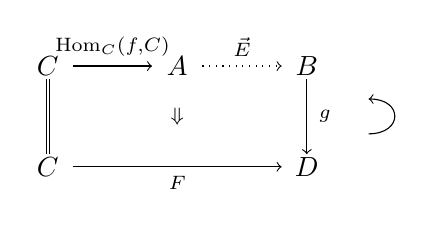
\begin{tikzpicture}[x=1.3em,y=1.3em]
  \node (s2a) at (0,1.4)   {$C$};
  \node (s2b) at (3.6,1.4) {$A$};
  \node (s2c) at (7.2,1.4) {$B$};
  \node (s2d) at (0,-1.4)  {$C$};
  \node (s2e) at (7.2,-1.4){$D$};
  \draw[->] (0.7,1.4) -- node[above]{$\scriptstyle\HomC(f,C)$} (2.9,1.4);
  \draw[->,dotted] (4.3,1.4) -- node[above]{$\scriptstyle\vec{E}$} (6.5,1.4);
  \draw[double,double distance=0.6pt] (0,1.05) -- (0,-1.05);
  \draw[->] (7.2,1.05) -- (7.2,-1.05);
  \node at (7.7,0) {$\scriptstyle g$};
  \node at (3.6,0) {$\scriptstyle\Downarrow$};
  \node at (9.4,0) {$\rvbendR$};
  \draw[->] (0.7,-1.4) -- node[below]{$\scriptstyle F$} (6.5,-1.4);
\end{tikzpicture}
\qquad
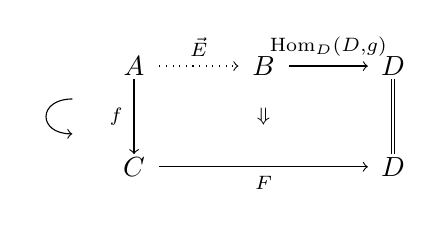
\begin{tikzpicture}[x=1.3em,y=1.3em]
  \node at (-2.2,0) {$\rvbendL$};
  \node (s3a) at (0,1.4)   {$A$};
  \node (s3b) at (3.6,1.4) {$B$};
  \node (s3c) at (7.2,1.4) {$D$};
  \node (s3d) at (0,-1.4)  {$C$};
  \node (s3e) at (7.2,-1.4){$D$};
  \draw[->,dotted] (0.7,1.4) -- node[above]{$\scriptstyle\vec{E}$} (2.9,1.4);
  \draw[->] (4.3,1.4) -- node[above]{$\scriptstyle\HomD(D,g)$} (6.5,1.4);
  \draw[->] (0,1.05) -- (0,-1.05);
  \node at (-0.5,0) {$\scriptstyle f$};
  \draw[double,double distance=0.6pt] (7.2,1.05) -- (7.2,-1.05);
  \node at (3.6,0) {$\scriptstyle\Downarrow$};
  \draw[->] (0.7,-1.4) -- node[below]{$\scriptstyle F$} (6.5,-1.4);
\end{tikzpicture}
\\[1.2em]
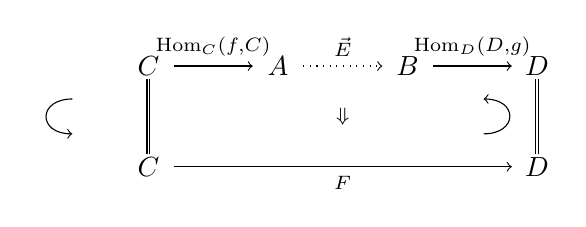
\begin{tikzpicture}[x=1.3em,y=1.3em]
  \node at (-2.6,0) {$\rvbendL$};
  \node at (9.8,0)  {$\rvbendR$};
  \node (s4a) at (0,1.4)    {$C$};
  \node (s4b) at (3.6,1.4)  {$A$};
  \node (s4c) at (7.2,1.4)  {$B$};
  \node (s4d) at (10.8,1.4) {$D$};
  \node (s4e) at (0,-1.4)   {$C$};
  \node (s4f) at (10.8,-1.4){$D$};
  \draw[->] (0.7,1.4) -- node[above]{$\scriptstyle\HomC(f,C)$} (2.9,1.4);
  \draw[->,dotted] (4.3,1.4) -- node[above]{$\scriptstyle\vec{E}$} (6.5,1.4);
  \draw[->] (7.9,1.4) -- node[above]{$\scriptstyle\HomD(D,g)$} (10.1,1.4);
  \draw[double,double distance=0.6pt] (0,1.05) -- (0,-1.05);
  \draw[double,double distance=0.6pt] (10.8,1.05) -- (10.8,-1.05);
  \node at (5.4,0) {$\scriptstyle\Downarrow$};
  \draw[->] (0.7,-1.4) -- node[below]{$\scriptstyle F$} (10.1,-1.4);
\end{tikzpicture}
\end{center}
\end{theorem}

\begin{proof}
陈述中纵向排出的那个复合双射，把胞腔 $\alpha$ 与 $\beta$ 分别送到下左图与下右图
所示的胞腔：
\begin{center}
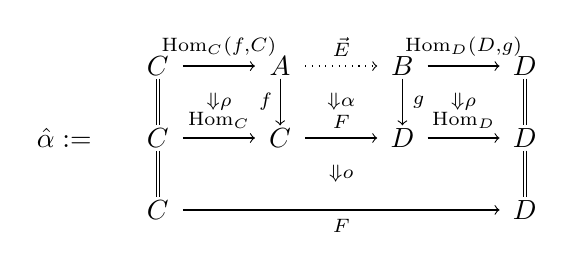
\begin{tikzpicture}[x=1.3em,y=1.3em]
  \node at (-2.6,0.6) {$\hat{\alpha}:=$};
  \node (aa1) at (0,2.6)    {$C$};
  \node (aa2) at (3.4,2.6)  {$A$};
  \node (aa3) at (6.8,2.6)  {$B$};
  \node (aa4) at (10.2,2.6) {$D$};
  \node (aa5) at (0,0.6)    {$C$};
  \node (aa6) at (3.4,0.6)  {$C$};
  \node (aa7) at (6.8,0.6)  {$D$};
  \node (aa8) at (10.2,0.6) {$D$};
  \node (aa9) at (0,-1.4)   {$C$};
  \node (aa10) at (10.2,-1.4){$D$};
  \draw[->] (0.7,2.6) -- node[above]{$\scriptstyle\HomC(f,C)$} (2.7,2.6);
  \draw[->,dotted] (4.1,2.6) -- node[above]{$\scriptstyle\vec{E}$} (6.1,2.6);
  \draw[->] (7.5,2.6) -- node[above]{$\scriptstyle\HomD(D,g)$} (9.5,2.6);
  \draw[->] (0.7,0.6) -- node[above]{$\scriptstyle\HomC$} (2.7,0.6);
  \draw[->] (4.1,0.6) -- node[above]{$\scriptstyle F$} (6.1,0.6);
  \draw[->] (7.5,0.6) -- node[above]{$\scriptstyle\HomD$} (9.5,0.6);
  \draw[->] (0.7,-1.4) -- node[below]{$\scriptstyle F$} (9.5,-1.4);
  \draw[double,double distance=0.6pt] (0,2.25) -- (0,0.95);
  \draw[->] (3.4,2.25) -- (3.4,0.95);
  \node at (3.0,1.6) {$\scriptstyle f$};
  \draw[->] (6.8,2.25) -- (6.8,0.95);
  \node at (7.25,1.6) {$\scriptstyle g$};
  \draw[double,double distance=0.6pt] (10.2,2.25) -- (10.2,0.95);
  \node at (1.7,1.6) {$\scriptstyle\Downarrow\rho$};
  \node at (5.1,1.6) {$\scriptstyle\Downarrow\alpha$};
  \node at (8.5,1.6) {$\scriptstyle\Downarrow\rho$};
  \draw[double,double distance=0.6pt] (0,0.25) -- (0,-1.05);
  \draw[double,double distance=0.6pt] (10.2,0.25) -- (10.2,-1.05);
  \node at (5.1,-0.4) {$\scriptstyle\Downarrow o$};
\end{tikzpicture}
\qquad
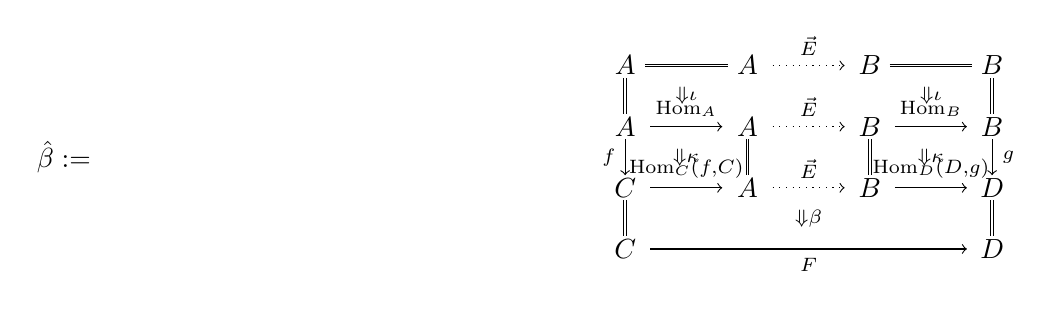
\begin{tikzpicture}[x=1.3em,y=1.3em]
  \node at (-2.6,0.85) {$\hat{\beta}:=$};
  \begin{scope}[shift={(13.0,0)}]
  \node (ba1) at (0,3.4)    {$A$};
  \node (ba2) at (3.4,3.4)  {$A$};
  \node (ba3) at (6.8,3.4)  {$B$};
  \node (ba4) at (10.2,3.4) {$B$};
  \node (ba5) at (0,1.7)    {$A$};
  \node (ba6) at (3.4,1.7)  {$A$};
  \node (ba7) at (6.8,1.7)  {$B$};
  \node (ba8) at (10.2,1.7) {$B$};
  \node (ba9) at (0,0)      {$C$};
  \node (ba10) at (3.4,0)   {$A$};
  \node (ba11) at (6.8,0)   {$B$};
  \node (ba12) at (10.2,0)  {$D$};
  \node (ba13) at (0,-1.7)  {$C$};
  \node (ba14) at (10.2,-1.7){$D$};
  \draw[double,double distance=0.6pt] (0.55,3.4) -- (2.85,3.4);
  \draw[->,dotted] (4.1,3.4) -- node[above]{$\scriptstyle\vec{E}$} (6.1,3.4);
  \draw[double,double distance=0.6pt] (7.35,3.4) -- (9.65,3.4);
  \draw[->] (0.7,1.7) -- node[above]{$\scriptstyle\HomA$} (2.7,1.7);
  \draw[->,dotted] (4.1,1.7) -- node[above]{$\scriptstyle\vec{E}$} (6.1,1.7);
  \draw[->] (7.5,1.7) -- node[above]{$\scriptstyle\HomB$} (9.5,1.7);
  \draw[->] (0.7,0) -- node[above]{$\scriptstyle\HomC(f,C)$} (2.7,0);
  \draw[->,dotted] (4.1,0) -- node[above]{$\scriptstyle\vec{E}$} (6.1,0);
  \draw[->] (7.5,0) -- node[above]{$\scriptstyle\HomD(D,g)$} (9.5,0);
  \draw[->] (0.7,-1.7) -- node[below]{$\scriptstyle F$} (9.5,-1.7);
  \draw[double,double distance=0.6pt] (0,3.05) -- (0,2.05);
  \node at (1.7,2.55) {$\scriptstyle\Downarrow\iota$};
  \node at (8.5,2.55) {$\scriptstyle\Downarrow\iota$};
  \draw[double,double distance=0.6pt] (10.2,3.05) -- (10.2,2.05);
  \draw[->] (0,1.35) -- (0,0.35);
  \node at (-0.45,0.85) {$\scriptstyle f$};
  \draw[double,double distance=0.6pt] (3.4,1.35) -- (3.4,0.35);
  \node at (1.7,0.85) {$\scriptstyle\Downarrow\kappa$};
  \draw[double,double distance=0.6pt] (6.8,1.35) -- (6.8,0.35);
  \node at (8.5,0.85) {$\scriptstyle\Downarrow\kappa$};
  \draw[->] (10.2,1.35) -- (10.2,0.35);
  \node at (10.65,0.85) {$\scriptstyle g$};
  \draw[double,double distance=0.6pt] (0,-0.35) -- (0,-1.35);
  \node at (5.1,-0.85) {$\scriptstyle\Downarrow\beta$};
  \draw[double,double distance=0.6pt] (10.2,-0.35) -- (10.2,-1.35);
  \end{scope}
\end{tikzpicture}
\end{center}
由\cref{prop:representable-restriction-application}与引理 8.3.15
\begin{center}
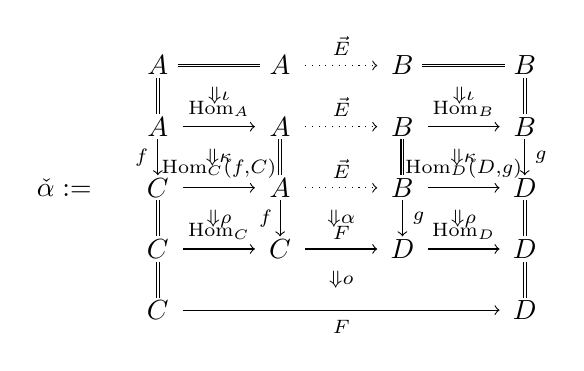
\begin{tikzpicture}[x=1.3em,y=1.3em]
  \node at (-2.6,2.6) {$\check{\alpha}:=$};
  \node (ca1) at (0,6.0)    {$A$};
  \node (ca2) at (3.4,6.0)  {$A$};
  \node (ca3) at (6.8,6.0)  {$B$};
  \node (ca4) at (10.2,6.0) {$B$};
  \node (ca5) at (0,4.3)    {$A$};
  \node (ca6) at (3.4,4.3)  {$A$};
  \node (ca7) at (6.8,4.3)  {$B$};
  \node (ca8) at (10.2,4.3) {$B$};
  \node (ca9) at (0,2.6)    {$C$};
  \node (ca10) at (3.4,2.6) {$A$};
  \node (ca11) at (6.8,2.6) {$B$};
  \node (ca12) at (10.2,2.6){$D$};
  \node (ca13) at (0,0.9)   {$C$};
  \node (ca14) at (3.4,0.9) {$C$};
  \node (ca15) at (6.8,0.9) {$D$};
  \node (ca16) at (10.2,0.9){$D$};
  \node (ca17) at (0,-0.8)  {$C$};
  \node (ca18) at (10.2,-0.8){$D$};
  \draw[double,double distance=0.6pt] (0.55,6.0) -- (2.85,6.0);
  \draw[->,dotted] (4.1,6.0) -- node[above]{$\scriptstyle\vec{E}$} (6.1,6.0);
  \draw[double,double distance=0.6pt] (7.35,6.0) -- (9.65,6.0);
  \draw[->] (0.7,4.3) -- node[above]{$\scriptstyle\HomA$} (2.7,4.3);
  \draw[->,dotted] (4.1,4.3) -- node[above]{$\scriptstyle\vec{E}$} (6.1,4.3);
  \draw[->] (7.5,4.3) -- node[above]{$\scriptstyle\HomB$} (9.5,4.3);
  \draw[->] (0.7,2.6) -- node[above]{$\scriptstyle\HomC(f,C)$} (2.7,2.6);
  \draw[->,dotted] (4.1,2.6) -- node[above]{$\scriptstyle\vec{E}$} (6.1,2.6);
  \draw[->] (7.5,2.6) -- node[above]{$\scriptstyle\HomD(D,g)$} (9.5,2.6);
  \draw[->] (0.7,0.9) -- node[above]{$\scriptstyle\HomC$} (2.7,0.9);
  \draw[->] (4.1,0.9) -- node[above]{$\scriptstyle F$} (6.1,0.9);
  \draw[->] (7.5,0.9) -- node[above]{$\scriptstyle\HomD$} (9.5,0.9);
  \draw[->] (0.7,-0.8) -- node[below]{$\scriptstyle F$} (9.5,-0.8);
  \draw[double,double distance=0.6pt] (0,5.65) -- (0,4.65);
  \node at (1.7,5.15) {$\scriptstyle\Downarrow\iota$};
  \node at (8.5,5.15) {$\scriptstyle\Downarrow\iota$};
  \draw[double,double distance=0.6pt] (10.2,5.65) -- (10.2,4.65);
  \draw[->] (0,3.95) -- (0,2.95);
  \node at (-0.45,3.45) {$\scriptstyle f$};
  \node at (1.7,3.45) {$\scriptstyle\Downarrow\kappa$};
  \draw[double,double distance=0.6pt] (3.4,3.95) -- (3.4,2.95);
  \draw[double,double distance=0.6pt] (6.8,3.95) -- (6.8,2.95);
  \node at (8.5,3.45) {$\scriptstyle\Downarrow\kappa$};
  \draw[->] (10.2,3.95) -- (10.2,2.95);
  \node at (10.65,3.45) {$\scriptstyle g$};
  \draw[double,double distance=0.6pt] (0,2.25) -- (0,1.25);
  \draw[->] (3.4,2.25) -- (3.4,1.25);
  \node at (3.0,1.75) {$\scriptstyle f$};
  \draw[->] (6.8,2.25) -- (6.8,1.25);
  \node at (7.25,1.75) {$\scriptstyle g$};
  \draw[double,double distance=0.6pt] (10.2,2.25) -- (10.2,1.25);
  \node at (1.7,1.75) {$\scriptstyle\Downarrow\rho$};
  \node at (5.1,1.75) {$\scriptstyle\Downarrow\alpha$};
  \node at (8.5,1.75) {$\scriptstyle\Downarrow\rho$};
  \draw[double,double distance=0.6pt] (0,0.55) -- (0,-0.45);
  \draw[double,double distance=0.6pt] (10.2,0.55) -- (10.2,-0.45);
  \node at (5.1,0.05) {$\scriptstyle\Downarrow o$};
\end{tikzpicture}
\qquad $=$ \qquad
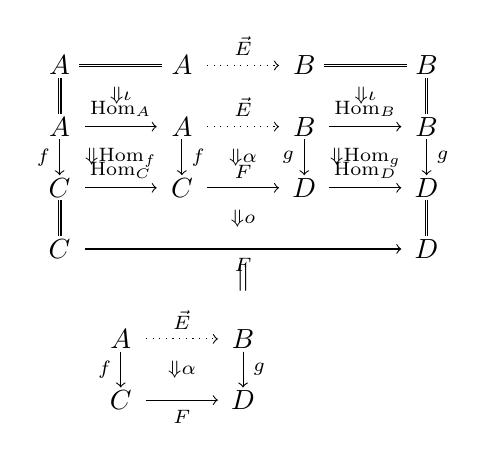
\begin{tikzpicture}[x=1.3em,y=1.3em]
  \begin{scope}[shift={(15.0,0)}]
  \node (da1) at (0,6.0)    {$A$};
  \node (da2) at (3.4,6.0)  {$A$};
  \node (da3) at (6.8,6.0)  {$B$};
  \node (da4) at (10.2,6.0) {$B$};
  \node (da5) at (0,4.3)    {$A$};
  \node (da6) at (3.4,4.3)  {$A$};
  \node (da7) at (6.8,4.3)  {$B$};
  \node (da8) at (10.2,4.3) {$B$};
  \node (da9) at (0,2.6)    {$C$};
  \node (da10) at (3.4,2.6) {$C$};
  \node (da11) at (6.8,2.6) {$D$};
  \node (da12) at (10.2,2.6){$D$};
  \node (da13) at (0,0.9)   {$C$};
  \node (da14) at (10.2,0.9){$D$};
  \draw[double,double distance=0.6pt] (0.55,6.0) -- (2.85,6.0);
  \draw[->,dotted] (4.1,6.0) -- node[above]{$\scriptstyle\vec{E}$} (6.1,6.0);
  \draw[double,double distance=0.6pt] (7.35,6.0) -- (9.65,6.0);
  \draw[->] (0.7,4.3) -- node[above]{$\scriptstyle\HomA$} (2.7,4.3);
  \draw[->,dotted] (4.1,4.3) -- node[above]{$\scriptstyle\vec{E}$} (6.1,4.3);
  \draw[->] (7.5,4.3) -- node[above]{$\scriptstyle\HomB$} (9.5,4.3);
  \draw[->] (0.7,2.6) -- node[above]{$\scriptstyle\HomC$} (2.7,2.6);
  \draw[->] (4.1,2.6) -- node[above]{$\scriptstyle F$} (6.1,2.6);
  \draw[->] (7.5,2.6) -- node[above]{$\scriptstyle\HomD$} (9.5,2.6);
  \draw[->] (0.7,0.9) -- node[below]{$\scriptstyle F$} (9.5,0.9);
  \draw[double,double distance=0.6pt] (0,5.65) -- (0,4.65);
  \node at (1.7,5.15) {$\scriptstyle\Downarrow\iota$};
  \node at (8.5,5.15) {$\scriptstyle\Downarrow\iota$};
  \draw[double,double distance=0.6pt] (10.2,5.65) -- (10.2,4.65);
  \draw[->] (0,3.95) -- (0,2.95);
  \node at (-0.45,3.45) {$\scriptstyle f$};
  \node at (1.7,3.45) {$\scriptstyle\Downarrow\mathrm{Hom}_{f}$};
  \draw[->] (3.4,3.95) -- (3.4,2.95);
  \node at (3.85,3.45) {$\scriptstyle f$};
  \node at (5.1,3.45) {$\scriptstyle\Downarrow\alpha$};
  \draw[->] (6.8,3.95) -- (6.8,2.95);
  \node at (6.35,3.45) {$\scriptstyle g$};
  \node at (8.5,3.45) {$\scriptstyle\Downarrow\mathrm{Hom}_{g}$};
  \draw[->] (10.2,3.95) -- (10.2,2.95);
  \node at (10.65,3.45) {$\scriptstyle g$};
  \draw[double,double distance=0.6pt] (0,2.25) -- (0,1.25);
  \draw[double,double distance=0.6pt] (10.2,2.25) -- (10.2,1.25);
  \node at (5.1,1.75) {$\scriptstyle\Downarrow o$};
  \node at (5.1,0.1) {$\Vert$};
  \node (ea1) at (1.7,-1.6)  {$A$};
  \node (ea2) at (5.1,-1.6)  {$B$};
  \node (ea3) at (1.7,-3.3)  {$C$};
  \node (ea4) at (5.1,-3.3)  {$D$};
  \draw[->,dotted] (2.4,-1.6) -- node[above]{$\scriptstyle\vec{E}$} (4.4,-1.6);
  \draw[->] (1.7,-1.95) -- (1.7,-2.95);
  \node at (1.25,-2.45) {$\scriptstyle f$};
  \draw[->] (5.1,-1.95) -- (5.1,-2.95);
  \node at (5.55,-2.45) {$\scriptstyle g$};
  \node at (3.4,-2.45) {$\scriptstyle\Downarrow\alpha$};
  \draw[->] (2.4,-3.3) -- node[below]{$\scriptstyle F$} (4.4,-3.3);
  \end{scope}
\end{tikzpicture}
\end{center}

另一个复合是：
\begin{rveq}\label{eq:beta-image}
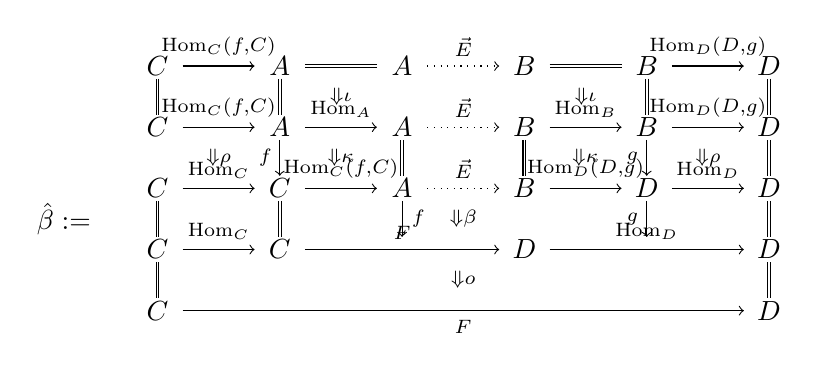
\begin{tikzpicture}[x=1.3em,y=1.3em]
  \node at (-2.6,2.55) {$\hat{\beta}:=$};
  \node (fa1) at (0,6.8)    {$C$};
  \node (fa2) at (3.4,6.8)  {$A$};
  \node (fa3) at (6.8,6.8)  {$A$};
  \node (fa4) at (10.2,6.8) {$B$};
  \node (fa5) at (13.6,6.8) {$B$};
  \node (fa6) at (17.0,6.8) {$D$};
  \node (fa7) at (0,5.1)    {$C$};
  \node (fa8) at (3.4,5.1)  {$A$};
  \node (fa9) at (6.8,5.1)  {$A$};
  \node (fa10) at (10.2,5.1){$B$};
  \node (fa11) at (13.6,5.1){$B$};
  \node (fa12) at (17.0,5.1){$D$};
  \node (fa13) at (0,3.4)   {$C$};
  \node (fa14) at (3.4,3.4) {$C$};
  \node (fa15) at (6.8,3.4) {$A$};
  \node (fa16) at (10.2,3.4){$B$};
  \node (fa17) at (13.6,3.4){$D$};
  \node (fa18) at (17.0,3.4){$D$};
  \node (fa19) at (0,1.7)   {$C$};
  \node (fa20) at (3.4,1.7) {$C$};
  \node (fa21) at (10.2,1.7){$D$};
  \node (fa22) at (17.0,1.7){$D$};
  \node (fa23) at (0,0)     {$C$};
  \node (fa24) at (17.0,0)  {$D$};
  \draw[->] (0.7,6.8) -- node[above]{$\scriptstyle\HomC(f,C)$} (2.7,6.8);
  \draw[double,double distance=0.6pt] (4.1,6.8) -- (6.1,6.8);
  \draw[->,dotted] (7.5,6.8) -- node[above]{$\scriptstyle\vec{E}$} (9.5,6.8);
  \draw[double,double distance=0.6pt] (10.9,6.8) -- (12.9,6.8);
  \draw[->] (14.3,6.8) -- node[above]{$\scriptstyle\HomD(D,g)$} (16.3,6.8);
  \draw[->] (0.7,5.1) -- node[above]{$\scriptstyle\HomC(f,C)$} (2.7,5.1);
  \draw[->] (4.1,5.1) -- node[above]{$\scriptstyle\HomA$} (6.1,5.1);
  \draw[->,dotted] (7.5,5.1) -- node[above]{$\scriptstyle\vec{E}$} (9.5,5.1);
  \draw[->] (10.9,5.1) -- node[above]{$\scriptstyle\HomB$} (12.9,5.1);
  \draw[->] (14.3,5.1) -- node[above]{$\scriptstyle\HomD(D,g)$} (16.3,5.1);
  \draw[->] (0.7,3.4) -- node[above]{$\scriptstyle\HomC$} (2.7,3.4);
  \draw[->] (4.1,3.4) -- node[above]{$\scriptstyle\HomC(f,C)$} (6.1,3.4);
  \draw[->,dotted] (7.5,3.4) -- node[above]{$\scriptstyle\vec{E}$} (9.5,3.4);
  \draw[->] (10.9,3.4) -- node[above]{$\scriptstyle\HomD(D,g)$} (12.9,3.4);
  \draw[->] (14.3,3.4) -- node[above]{$\scriptstyle\HomD$} (16.3,3.4);
  \draw[->] (0.7,1.7) -- node[above]{$\scriptstyle\HomC$} (2.7,1.7);
  \draw[->] (4.1,1.7) -- node[above]{$\scriptstyle F$} (9.5,1.7);
  \draw[->] (10.9,1.7) -- node[above]{$\scriptstyle\HomD$} (16.3,1.7);
  \draw[->] (0.7,0) -- node[below]{$\scriptstyle F$} (16.3,0);
  \draw[double,double distance=0.6pt] (0,6.45) -- (0,5.45);
  \draw[double,double distance=0.6pt] (3.4,6.45) -- (3.4,5.45);
  \node at (5.1,5.95) {$\scriptstyle\Downarrow\iota$};
  \node at (11.9,5.95) {$\scriptstyle\Downarrow\iota$};
  \draw[double,double distance=0.6pt] (13.6,6.45) -- (13.6,5.45);
  \draw[double,double distance=0.6pt] (17.0,6.45) -- (17.0,5.45);
  \node at (1.7,4.25) {$\scriptstyle\Downarrow\rho$};
  \draw[->] (3.4,4.75) -- (3.4,3.75);
  \node at (3.0,4.25) {$\scriptstyle f$};
  \node at (5.1,4.25) {$\scriptstyle\Downarrow\kappa$};
  \draw[double,double distance=0.6pt] (6.8,4.75) -- (6.8,3.75);
  \draw[double,double distance=0.6pt] (10.2,4.75) -- (10.2,3.75);
  \node at (11.9,4.25) {$\scriptstyle\Downarrow\kappa$};
  \draw[->] (13.6,4.75) -- (13.6,3.75);
  \node at (13.2,4.25) {$\scriptstyle g$};
  \node at (15.3,4.25) {$\scriptstyle\Downarrow\rho$};
  \draw[double,double distance=0.6pt] (17.0,4.75) -- (17.0,3.75);
  \draw[double,double distance=0.6pt] (0,3.05) -- (0,2.05);
  \draw[double,double distance=0.6pt] (3.4,3.05) -- (3.4,2.05);
  \draw[->] (6.8,3.05) -- (6.8,2.05);
  \node at (7.25,2.55) {$\scriptstyle f$};
  \draw[->] (13.6,3.05) -- (13.6,2.05);
  \node at (13.2,2.55) {$\scriptstyle g$};
  \draw[double,double distance=0.6pt] (17.0,3.05) -- (17.0,2.05);
  \node at (8.5,2.55) {$\scriptstyle\Downarrow\beta$};
  \draw[double,double distance=0.6pt] (0,1.35) -- (0,0.35);
  \draw[double,double distance=0.6pt] (17.0,1.35) -- (17.0,0.35);
  \node at (8.5,0.85) {$\scriptstyle\Downarrow o$};
\end{tikzpicture}
\end{rveq}
由引理 8.3.10，我们有
\begin{center}
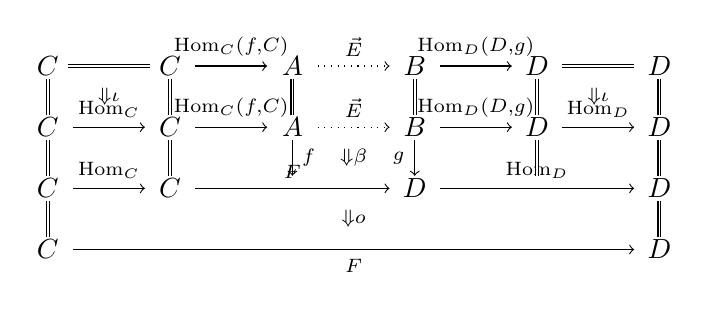
\begin{tikzpicture}[x=1.3em,y=1.3em]
  \node (ga1) at (0,5.4)    {$C$};
  \node (ga2) at (3.4,5.4)  {$C$};
  \node (ga3) at (6.8,5.4)  {$A$};
  \node (ga4) at (10.2,5.4) {$B$};
  \node (ga5) at (13.6,5.4) {$D$};
  \node (ga6) at (17.0,5.4) {$D$};
  \node (ga7) at (0,3.7)    {$C$};
  \node (ga8) at (3.4,3.7)  {$C$};
  \node (ga9) at (6.8,3.7)  {$A$};
  \node (ga10) at (10.2,3.7){$B$};
  \node (ga11) at (13.6,3.7){$D$};
  \node (ga12) at (17.0,3.7){$D$};
  \node (ga13) at (0,2.0)   {$C$};
  \node (ga14) at (3.4,2.0) {$C$};
  \node (ga15) at (10.2,2.0){$D$};
  \node (ga16) at (17.0,2.0){$D$};
  \node (ga17) at (0,0.3)   {$C$};
  \node (ga18) at (17.0,0.3){$D$};
  \draw[double,double distance=0.6pt] (0.55,5.4) -- (2.85,5.4);
  \draw[->] (4.1,5.4) -- node[above]{$\scriptstyle\HomC(f,C)$} (6.1,5.4);
  \draw[->,dotted] (7.5,5.4) -- node[above]{$\scriptstyle\vec{E}$} (9.5,5.4);
  \draw[->] (10.9,5.4) -- node[above]{$\scriptstyle\HomD(D,g)$} (12.9,5.4);
  \draw[double,double distance=0.6pt] (14.3,5.4) -- (16.3,5.4);
  \draw[->] (0.7,3.7) -- node[above]{$\scriptstyle\HomC$} (2.7,3.7);
  \draw[->] (4.1,3.7) -- node[above]{$\scriptstyle\HomC(f,C)$} (6.1,3.7);
  \draw[->,dotted] (7.5,3.7) -- node[above]{$\scriptstyle\vec{E}$} (9.5,3.7);
  \draw[->] (10.9,3.7) -- node[above]{$\scriptstyle\HomD(D,g)$} (12.9,3.7);
  \draw[->] (14.3,3.7) -- node[above]{$\scriptstyle\HomD$} (16.3,3.7);
  \draw[->] (0.7,2.0) -- node[above]{$\scriptstyle\HomC$} (2.7,2.0);
  \draw[->] (4.1,2.0) -- node[above]{$\scriptstyle F$} (9.5,2.0);
  \draw[->] (10.9,2.0) -- node[above]{$\scriptstyle\HomD$} (16.3,2.0);
  \draw[->] (0.7,0.3) -- node[below]{$\scriptstyle F$} (16.3,0.3);
  \node at (1.7,4.55) {$\scriptstyle\Downarrow\iota$};
  \draw[double,double distance=0.6pt] (0,5.05) -- (0,4.05);
  \draw[double,double distance=0.6pt] (3.4,5.05) -- (3.4,4.05);
  \draw[double,double distance=0.6pt] (6.8,5.05) -- (6.8,4.05);
  \draw[double,double distance=0.6pt] (10.2,5.05) -- (10.2,4.05);
  \node at (15.3,4.55) {$\scriptstyle\Downarrow\iota$};
  \draw[double,double distance=0.6pt] (13.6,5.05) -- (13.6,4.05);
  \draw[double,double distance=0.6pt] (17.0,5.05) -- (17.0,4.05);
  \node at (8.5,2.85) {$\scriptstyle\Downarrow\beta$};
  \draw[double,double distance=0.6pt] (0,3.35) -- (0,2.35);
  \draw[double,double distance=0.6pt] (3.4,3.35) -- (3.4,2.35);
  \draw[->] (6.8,3.35) -- (6.8,2.35);
  \node at (7.25,2.85) {$\scriptstyle f$};
  \draw[->] (10.2,3.35) -- (10.2,2.35);
  \node at (9.75,2.85) {$\scriptstyle g$};
  \draw[double,double distance=0.6pt] (13.6,3.35) -- (13.6,2.35);
  \draw[double,double distance=0.6pt] (17.0,3.35) -- (17.0,2.35);
  \node at (8.5,1.15) {$\scriptstyle\Downarrow o$};
  \draw[double,double distance=0.6pt] (0,1.65) -- (0,0.65);
  \draw[double,double distance=0.6pt] (17.0,1.65) -- (17.0,0.65);
\end{tikzpicture}
\\[1.0em]
$\Vert$
\\[1.0em]
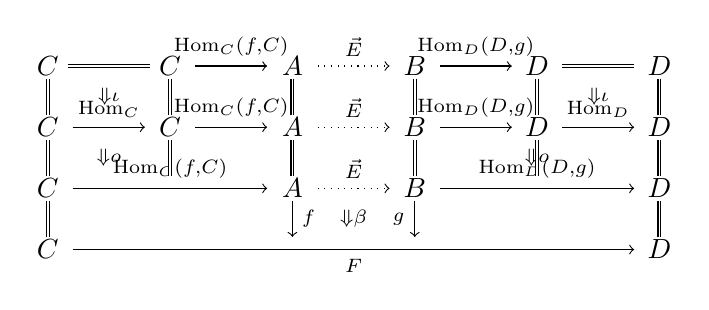
\begin{tikzpicture}[x=1.3em,y=1.3em]
  \node (ha1) at (0,5.4)    {$C$};
  \node (ha2) at (3.4,5.4)  {$C$};
  \node (ha3) at (6.8,5.4)  {$A$};
  \node (ha4) at (10.2,5.4) {$B$};
  \node (ha5) at (13.6,5.4) {$D$};
  \node (ha6) at (17.0,5.4) {$D$};
  \node (ha7) at (0,3.7)    {$C$};
  \node (ha8) at (3.4,3.7)  {$C$};
  \node (ha9) at (6.8,3.7)  {$A$};
  \node (ha10) at (10.2,3.7){$B$};
  \node (ha11) at (13.6,3.7){$D$};
  \node (ha12) at (17.0,3.7){$D$};
  \node (ha13) at (0,2.0)   {$C$};
  \node (ha14) at (6.8,2.0) {$A$};
  \node (ha15) at (10.2,2.0){$B$};
  \node (ha16) at (17.0,2.0){$D$};
  \node (ha17) at (0,0.3)   {$C$};
  \node (ha18) at (17.0,0.3){$D$};
  \draw[double,double distance=0.6pt] (0.55,5.4) -- (2.85,5.4);
  \draw[->] (4.1,5.4) -- node[above]{$\scriptstyle\HomC(f,C)$} (6.1,5.4);
  \draw[->,dotted] (7.5,5.4) -- node[above]{$\scriptstyle\vec{E}$} (9.5,5.4);
  \draw[->] (10.9,5.4) -- node[above]{$\scriptstyle\HomD(D,g)$} (12.9,5.4);
  \draw[double,double distance=0.6pt] (14.3,5.4) -- (16.3,5.4);
  \draw[->] (0.7,3.7) -- node[above]{$\scriptstyle\HomC$} (2.7,3.7);
  \draw[->] (4.1,3.7) -- node[above]{$\scriptstyle\HomC(f,C)$} (6.1,3.7);
  \draw[->,dotted] (7.5,3.7) -- node[above]{$\scriptstyle\vec{E}$} (9.5,3.7);
  \draw[->] (10.9,3.7) -- node[above]{$\scriptstyle\HomD(D,g)$} (12.9,3.7);
  \draw[->] (14.3,3.7) -- node[above]{$\scriptstyle\HomD$} (16.3,3.7);
  \draw[->] (0.7,2.0) -- node[above]{$\scriptstyle\HomC(f,C)$} (6.1,2.0);
  \draw[->,dotted] (7.5,2.0) -- node[above]{$\scriptstyle\vec{E}$} (9.5,2.0);
  \draw[->] (10.9,2.0) -- node[above]{$\scriptstyle\HomD(D,g)$} (16.3,2.0);
  \draw[->] (0.7,0.3) -- node[below]{$\scriptstyle F$} (16.3,0.3);
  \node at (1.7,4.55) {$\scriptstyle\Downarrow\iota$};
  \draw[double,double distance=0.6pt] (0,5.05) -- (0,4.05);
  \draw[double,double distance=0.6pt] (3.4,5.05) -- (3.4,4.05);
  \draw[double,double distance=0.6pt] (6.8,5.05) -- (6.8,4.05);
  \draw[double,double distance=0.6pt] (10.2,5.05) -- (10.2,4.05);
  \node at (15.3,4.55) {$\scriptstyle\Downarrow\iota$};
  \draw[double,double distance=0.6pt] (13.6,5.05) -- (13.6,4.05);
  \draw[double,double distance=0.6pt] (17.0,5.05) -- (17.0,4.05);
  \node at (1.7,2.85) {$\scriptstyle\Downarrow o$};
  \node at (13.6,2.85) {$\scriptstyle\Downarrow o$};
  \draw[double,double distance=0.6pt] (0,3.35) -- (0,2.35);
  \draw[double,double distance=0.6pt] (3.4,3.35) -- (3.4,2.35);
  \draw[double,double distance=0.6pt] (6.8,3.35) -- (6.8,2.35);
  \draw[double,double distance=0.6pt] (10.2,3.35) -- (10.2,2.35);
  \draw[double,double distance=0.6pt] (13.6,3.35) -- (13.6,2.35);
  \draw[double,double distance=0.6pt] (17.0,3.35) -- (17.0,2.35);
  \node at (8.5,1.15) {$\scriptstyle\Downarrow\beta$};
  \draw[double,double distance=0.6pt] (0,1.65) -- (0,0.65);
  \draw[->] (6.8,1.65) -- (6.8,0.65);
  \node at (7.25,1.15) {$\scriptstyle f$};
  \draw[->] (10.2,1.65) -- (10.2,0.65);
  \node at (9.75,1.15) {$\scriptstyle g$};
  \draw[double,double distance=0.6pt] (17.0,1.65) -- (17.0,0.65);
\end{tikzpicture}
\end{center}
由于这两个复合都等于 $\hat{\beta}$\footnote{原书此句印作「both composites
equal $\beta$」，无尖符。按文义，这两个复合所相等者是 $\beta$ 经双射所得之
像 $\hat{\beta}$（与本证明各图标签一致），疑原书脱尖符，此处径补。——译者注}。由命题 8.2.4 中诸单位胞腔的%
\trUniversalProperty{}，这些图表的下面两行相等，于是我们可以用右图的下面两行
替换 \eqref{eq:beta-image} 的下面两行，而得到：

\begin{center}
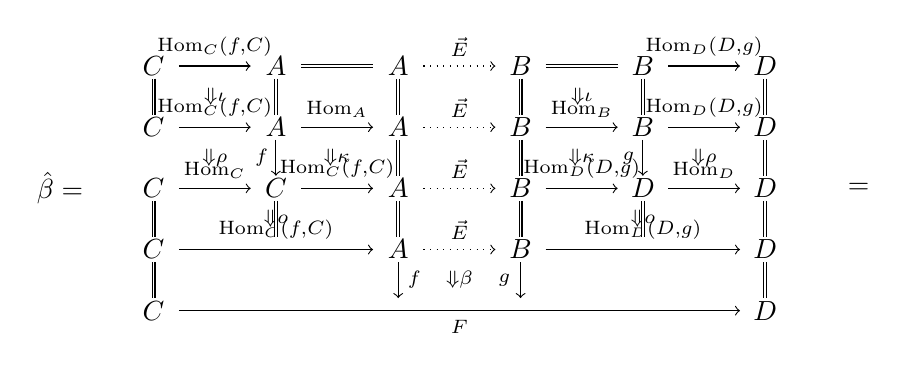
\begin{tikzpicture}[x=1.3em,y=1.3em]
  \node at (-2.6,3.4) {$\hat{\beta}=$};
  \node (ia1) at (0,6.8)    {$C$};
  \node (ia2) at (3.4,6.8)  {$A$};
  \node (ia3) at (6.8,6.8)  {$A$};
  \node (ia4) at (10.2,6.8) {$B$};
  \node (ia5) at (13.6,6.8) {$B$};
  \node (ia6) at (17.0,6.8) {$D$};
  \node (ia7) at (0,5.1)    {$C$};
  \node (ia8) at (3.4,5.1)  {$A$};
  \node (ia9) at (6.8,5.1)  {$A$};
  \node (ia10) at (10.2,5.1){$B$};
  \node (ia11) at (13.6,5.1){$B$};
  \node (ia12) at (17.0,5.1){$D$};
  \node (ia13) at (0,3.4)   {$C$};
  \node (ia14) at (3.4,3.4) {$C$};
  \node (ia15) at (6.8,3.4) {$A$};
  \node (ia16) at (10.2,3.4){$B$};
  \node (ia17) at (13.6,3.4){$D$};
  \node (ia18) at (17.0,3.4){$D$};
  \node (ia19) at (0,1.7)   {$C$};
  \node (ia20) at (6.8,1.7) {$A$};
  \node (ia21) at (10.2,1.7){$B$};
  \node (ia22) at (17.0,1.7){$D$};
  \node (ia23) at (0,0)     {$C$};
  \node (ia24) at (17.0,0)  {$D$};
  \draw[->] (0.7,6.8) -- node[above]{$\scriptstyle\HomC(f,C)$} (2.7,6.8);
  \draw[double,double distance=0.6pt] (4.1,6.8) -- (6.1,6.8);
  \draw[->,dotted] (7.5,6.8) -- node[above]{$\scriptstyle\vec{E}$} (9.5,6.8);
  \draw[double,double distance=0.6pt] (10.9,6.8) -- (12.9,6.8);
  \draw[->] (14.3,6.8) -- node[above]{$\scriptstyle\HomD(D,g)$} (16.3,6.8);
  \draw[->] (0.7,5.1) -- node[above]{$\scriptstyle\HomC(f,C)$} (2.7,5.1);
  \draw[->] (4.1,5.1) -- node[above]{$\scriptstyle\HomA$} (6.1,5.1);
  \draw[->,dotted] (7.5,5.1) -- node[above]{$\scriptstyle\vec{E}$} (9.5,5.1);
  \draw[->] (10.9,5.1) -- node[above]{$\scriptstyle\HomB$} (12.9,5.1);
  \draw[->] (14.3,5.1) -- node[above]{$\scriptstyle\HomD(D,g)$} (16.3,5.1);
  \draw[->] (0.7,3.4) -- node[above]{$\scriptstyle\HomC$} (2.7,3.4);
  \draw[->] (4.1,3.4) -- node[above]{$\scriptstyle\HomC(f,C)$} (6.1,3.4);
  \draw[->,dotted] (7.5,3.4) -- node[above]{$\scriptstyle\vec{E}$} (9.5,3.4);
  \draw[->] (10.9,3.4) -- node[above]{$\scriptstyle\HomD(D,g)$} (12.9,3.4);
  \draw[->] (14.3,3.4) -- node[above]{$\scriptstyle\HomD$} (16.3,3.4);
  \draw[->] (0.7,1.7) -- node[above]{$\scriptstyle\HomC(f,C)$} (6.1,1.7);
  \draw[->,dotted] (7.5,1.7) -- node[above]{$\scriptstyle\vec{E}$} (9.5,1.7);
  \draw[->] (10.9,1.7) -- node[above]{$\scriptstyle\HomD(D,g)$} (16.3,1.7);
  \draw[->] (0.7,0) -- node[below]{$\scriptstyle F$} (16.3,0);
  \node at (1.7,5.95) {$\scriptstyle\Downarrow\iota$};
  \draw[double,double distance=0.6pt] (0,6.45) -- (0,5.45);
  \draw[double,double distance=0.6pt] (3.4,6.45) -- (3.4,5.45);
  \draw[double,double distance=0.6pt] (6.8,6.45) -- (6.8,5.45);
  \draw[double,double distance=0.6pt] (10.2,6.45) -- (10.2,5.45);
  \node at (11.9,5.95) {$\scriptstyle\Downarrow\iota$};
  \draw[double,double distance=0.6pt] (13.6,6.45) -- (13.6,5.45);
  \draw[double,double distance=0.6pt] (17.0,6.45) -- (17.0,5.45);
  \node at (1.7,4.25) {$\scriptstyle\Downarrow\rho$};
  \draw[->] (3.4,4.75) -- (3.4,3.75);
  \node at (3.0,4.25) {$\scriptstyle f$};
  \node at (5.1,4.25) {$\scriptstyle\Downarrow\kappa$};
  \draw[double,double distance=0.6pt] (6.8,4.75) -- (6.8,3.75);
  \draw[double,double distance=0.6pt] (10.2,4.75) -- (10.2,3.75);
  \node at (11.9,4.25) {$\scriptstyle\Downarrow\kappa$};
  \draw[->] (13.6,4.75) -- (13.6,3.75);
  \node at (13.2,4.25) {$\scriptstyle g$};
  \node at (15.3,4.25) {$\scriptstyle\Downarrow\rho$};
  \draw[double,double distance=0.6pt] (17.0,4.75) -- (17.0,3.75);
  \node at (3.4,2.55) {$\scriptstyle\Downarrow o$};
  \node at (13.6,2.55) {$\scriptstyle\Downarrow o$};
  \draw[double,double distance=0.6pt] (0,3.05) -- (0,2.05);
  \draw[double,double distance=0.6pt] (3.4,3.05) -- (3.4,2.05);
  \draw[double,double distance=0.6pt] (6.8,3.05) -- (6.8,2.05);
  \draw[double,double distance=0.6pt] (10.2,3.05) -- (10.2,2.05);
  \draw[double,double distance=0.6pt] (13.6,3.05) -- (13.6,2.05);
  \draw[double,double distance=0.6pt] (17.0,3.05) -- (17.0,2.05);
  \node at (8.5,0.85) {$\scriptstyle\Downarrow\beta$};
  \draw[double,double distance=0.6pt] (0,1.35) -- (0,0.35);
  \draw[->] (6.8,1.35) -- (6.8,0.35);
  \node at (7.25,0.85) {$\scriptstyle f$};
  \draw[->] (10.2,1.35) -- (10.2,0.35);
  \node at (9.75,0.85) {$\scriptstyle g$};
  \draw[double,double distance=0.6pt] (17.0,1.35) -- (17.0,0.35);
  \node at (19.6,3.4) {$=$};
\end{tikzpicture}
\end{center}
由\cref{prop:representable-restriction-application}与引理 8.3.10，这就化归为
$\beta$。
\begin{center}
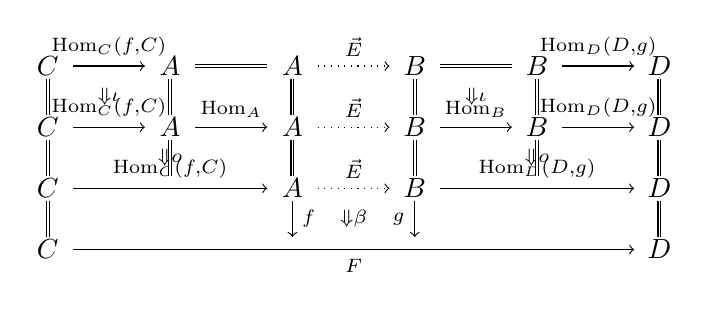
\begin{tikzpicture}[x=1.3em,y=1.3em]
  \node (ja1) at (0,5.4)    {$C$};
  \node (ja2) at (3.4,5.4)  {$A$};
  \node (ja3) at (6.8,5.4)  {$A$};
  \node (ja4) at (10.2,5.4) {$B$};
  \node (ja5) at (13.6,5.4) {$B$};
  \node (ja6) at (17.0,5.4) {$D$};
  \node (ja7) at (0,3.7)    {$C$};
  \node (ja8) at (3.4,3.7)  {$A$};
  \node (ja9) at (6.8,3.7)  {$A$};
  \node (ja10) at (10.2,3.7){$B$};
  \node (ja11) at (13.6,3.7){$B$};
  \node (ja12) at (17.0,3.7){$D$};
  \node (ja13) at (0,2.0)   {$C$};
  \node (ja14) at (6.8,2.0) {$A$};
  \node (ja15) at (10.2,2.0){$B$};
  \node (ja16) at (17.0,2.0){$D$};
  \node (ja17) at (0,0.3)   {$C$};
  \node (ja18) at (17.0,0.3){$D$};
  \draw[->] (0.7,5.4) -- node[above]{$\scriptstyle\HomC(f,C)$} (2.7,5.4);
  \draw[double,double distance=0.6pt] (4.1,5.4) -- (6.1,5.4);
  \draw[->,dotted] (7.5,5.4) -- node[above]{$\scriptstyle\vec{E}$} (9.5,5.4);
  \draw[double,double distance=0.6pt] (10.9,5.4) -- (12.9,5.4);
  \draw[->] (14.3,5.4) -- node[above]{$\scriptstyle\HomD(D,g)$} (16.3,5.4);
  \draw[->] (0.7,3.7) -- node[above]{$\scriptstyle\HomC(f,C)$} (2.7,3.7);
  \draw[->] (4.1,3.7) -- node[above]{$\scriptstyle\HomA$} (6.1,3.7);
  \draw[->,dotted] (7.5,3.7) -- node[above]{$\scriptstyle\vec{E}$} (9.5,3.7);
  \draw[->] (10.9,3.7) -- node[above]{$\scriptstyle\HomB$} (12.9,3.7);
  \draw[->] (14.3,3.7) -- node[above]{$\scriptstyle\HomD(D,g)$} (16.3,3.7);
  \draw[->] (0.7,2.0) -- node[above]{$\scriptstyle\HomC(f,C)$} (6.1,2.0);
  \draw[->,dotted] (7.5,2.0) -- node[above]{$\scriptstyle\vec{E}$} (9.5,2.0);
  \draw[->] (10.9,2.0) -- node[above]{$\scriptstyle\HomD(D,g)$} (16.3,2.0);
  \draw[->] (0.7,0.3) -- node[below]{$\scriptstyle F$} (16.3,0.3);
  \node at (1.7,4.55) {$\scriptstyle\Downarrow\iota$};
  \draw[double,double distance=0.6pt] (0,5.05) -- (0,4.05);
  \draw[double,double distance=0.6pt] (3.4,5.05) -- (3.4,4.05);
  \draw[double,double distance=0.6pt] (6.8,5.05) -- (6.8,4.05);
  \draw[double,double distance=0.6pt] (10.2,5.05) -- (10.2,4.05);
  \node at (11.9,4.55) {$\scriptstyle\Downarrow\iota$};
  \draw[double,double distance=0.6pt] (13.6,5.05) -- (13.6,4.05);
  \draw[double,double distance=0.6pt] (17.0,5.05) -- (17.0,4.05);
  \node at (3.4,2.85) {$\scriptstyle\Downarrow o$};
  \node at (13.6,2.85) {$\scriptstyle\Downarrow o$};
  \draw[double,double distance=0.6pt] (0,3.35) -- (0,2.35);
  \draw[double,double distance=0.6pt] (3.4,3.35) -- (3.4,2.35);
  \draw[double,double distance=0.6pt] (6.8,3.35) -- (6.8,2.35);
  \draw[double,double distance=0.6pt] (10.2,3.35) -- (10.2,2.35);
  \draw[double,double distance=0.6pt] (13.6,3.35) -- (13.6,2.35);
  \draw[double,double distance=0.6pt] (17.0,3.35) -- (17.0,2.35);
  \node at (8.5,1.15) {$\scriptstyle\Downarrow\beta$};
  \draw[double,double distance=0.6pt] (0,1.65) -- (0,0.65);
  \draw[->] (6.8,1.65) -- (6.8,0.65);
  \node at (7.25,1.15) {$\scriptstyle f$};
  \draw[->] (10.2,1.65) -- (10.2,0.65);
  \node at (9.75,1.15) {$\scriptstyle g$};
  \draw[double,double distance=0.6pt] (17.0,1.65) -- (17.0,0.65);
\end{tikzpicture}
\qquad $=$ \qquad
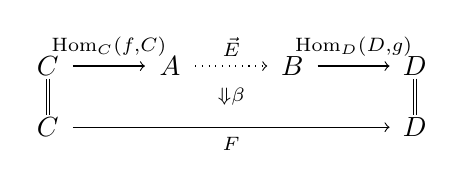
\begin{tikzpicture}[x=1.3em,y=1.3em]
  \begin{scope}[shift={(21.0,0)}]
  \node (ka1) at (0,2.0)    {$C$};
  \node (ka2) at (3.4,2.0)  {$A$};
  \node (ka3) at (6.8,2.0)  {$B$};
  \node (ka4) at (10.2,2.0) {$D$};
  \node (ka5) at (0,0.3)    {$C$};
  \node (ka6) at (10.2,0.3) {$D$};
  \draw[->] (0.7,2.0) -- node[above]{$\scriptstyle\HomC(f,C)$} (2.7,2.0);
  \draw[->,dotted] (4.1,2.0) -- node[above]{$\scriptstyle\vec{E}$} (6.1,2.0);
  \draw[->] (7.5,2.0) -- node[above]{$\scriptstyle\HomD(D,g)$} (9.5,2.0);
  \draw[->] (0.7,0.3) -- node[below]{$\scriptstyle F$} (9.5,0.3);
  \draw[double,double distance=0.6pt] (0,1.65) -- (0,0.65);
  \node at (5.1,1.15) {$\scriptstyle\Downarrow\beta$};
  \draw[double,double distance=0.6pt] (10.2,1.65) -- (10.2,0.65);
  \end{scope}
\end{tikzpicture}
\end{center}
对这个构造作竖直对分，即得陈述中的那些单侧双射。
\end{proof}

我们经常以下列形式使用这一结果：

\begin{corollary}\label{cor:compatible-sequence-bijection}
给定从 $A$ 到 $B$ 的一个相容\trModule{}序列
$E_{1}\divideontimes\cdots\divideontimes E_{n}$、从 $C$ 到 $D$ 的一个\trModule{} $F$，以及%
\trFunctor{} $f\colon A\to C$ 与 $g\colon B\to D$，在模的纤维化映射
$\HomC(f,C)\divideontimes E_{1}\divideontimes\cdots\divideontimes E_{n}\divideontimes\HomD(D,g)\Rightarrow F$
与模的纤维化映射 $E_{1}\divideontimes\cdots\divideontimes E_{n}\Rightarrow F(g,f)$ 之间，亦即
在如下两族胞腔之间存在一个双射：
\begin{center}
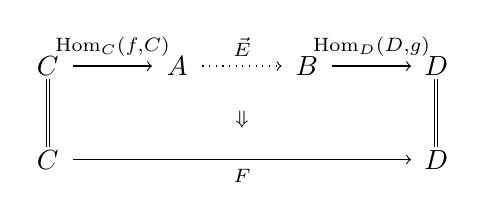
\begin{tikzpicture}[x=1.3em,y=1.3em]
  \node (la1) at (0,1.5)    {$C$};
  \node (la2) at (3.6,1.5)  {$A$};
  \node (la3) at (7.2,1.5)  {$B$};
  \node (la4) at (10.8,1.5) {$D$};
  \node (la5) at (0,-1.1)   {$C$};
  \node (la6) at (10.8,-1.1){$D$};
  \draw[->] (0.7,1.5) -- node[above]{$\scriptstyle\HomC(f,C)$} (2.9,1.5);
  \draw[->,dotted] (4.3,1.5) -- node[above]{$\scriptstyle\vec{E}$} (6.5,1.5);
  \draw[->] (7.9,1.5) -- node[above]{$\scriptstyle\HomD(D,g)$} (10.1,1.5);
  \draw[double,double distance=0.6pt] (0,1.15) -- (0,-0.75);
  \draw[double,double distance=0.6pt] (10.8,1.15) -- (10.8,-0.75);
  \node at (5.4,0) {$\scriptstyle\Downarrow$};
  \draw[->] (0.7,-1.1) -- node[below]{$\scriptstyle F$} (10.1,-1.1);
\end{tikzpicture}
\qquad $\mathrel{\leftrightsquigarrow}$ \qquad
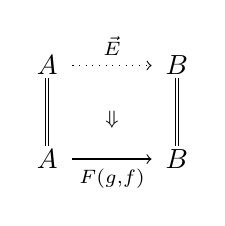
\begin{tikzpicture}[x=1.3em,y=1.3em]
  \node (ma1) at (0,1.5)  {$A$};
  \node (ma2) at (3.6,1.5){$B$};
  \node (ma3) at (0,-1.1) {$A$};
  \node (ma4) at (3.6,-1.1){$B$};
  \draw[->,dotted] (0.7,1.5) -- node[above]{$\scriptstyle\vec{E}$} (2.9,1.5);
  \draw[double,double distance=0.6pt] (0,1.15) -- (0,-0.75);
  \draw[double,double distance=0.6pt] (3.6,1.15) -- (3.6,-0.75);
  \node at (1.8,0) {$\scriptstyle\Downarrow$};
  \draw[->] (0.7,-1.1) -- node[below]{$\scriptstyle F(g,f)$} (2.9,-1.1);
\end{tikzpicture}
\end{center}
\end{corollary}

\begin{proof}
将\cref{thm:spider-lemma}与命题 8.2.1 结合起来。
\end{proof}

\begin{proposition}\label{prop:ternary-strong-composite}
对任意\trModule{} $A\xrightarrow{E}B$ 与一对\trFunctor{} $a\colon X\to A$、
$b\colon Y\to B$，强复合 $\HomA(A,a)\otimes E\otimes\HomB(b,B)$ 存在，且由限制
$E(b,a)$ 给出，其中三元强复合映射
$\mu\colon\HomA(A,a)\divideontimes E\divideontimes\HomB(b,B)\Rightarrow E(b,a)$ 由%
\trPastingDiagram{}所刻画的限制之\trUniversalProperty{}定义：
\begin{center}
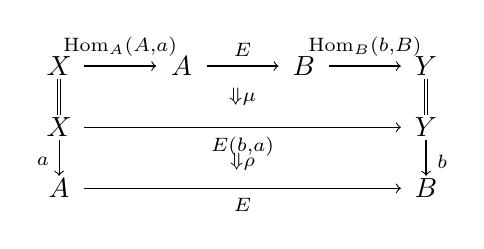
\begin{tikzpicture}[x=1.3em,y=1.3em]
  \node (na1) at (0,2.6)    {$X$};
  \node (na2) at (3.4,2.6)  {$A$};
  \node (na3) at (6.8,2.6)  {$B$};
  \node (na4) at (10.2,2.6) {$Y$};
  \node (na5) at (0,0.9)    {$X$};
  \node (na6) at (10.2,0.9) {$Y$};
  \node (na7) at (0,-0.8)   {$A$};
  \node (na8) at (10.2,-0.8){$B$};
  \draw[->] (0.7,2.6) -- node[above]{$\scriptstyle\HomA(A,a)$} (2.7,2.6);
  \draw[->] (4.1,2.6) -- node[above]{$\scriptstyle E$} (6.1,2.6);
  \draw[->] (7.5,2.6) -- node[above]{$\scriptstyle\HomB(b,B)$} (9.5,2.6);
  \draw[->] (0.7,0.9) -- node[below]{$\scriptstyle E(b,a)$} (9.5,0.9);
  \draw[->] (0.7,-0.8) -- node[below]{$\scriptstyle E$} (9.5,-0.8);
  \draw[double,double distance=0.6pt] (0,2.25) -- (0,1.25);
  \draw[double,double distance=0.6pt] (10.2,2.25) -- (10.2,1.25);
  \node at (5.1,1.75) {$\scriptstyle\Downarrow\mu$};
  \draw[->] (0,0.55) -- (0,-0.45);
  \node at (-0.45,-0.05) {$\scriptstyle a$};
  \draw[->] (10.2,0.55) -- (10.2,-0.45);
  \node at (10.65,-0.05) {$\scriptstyle b$};
  \node at (5.1,-0.05) {$\scriptstyle\Downarrow\rho$};
\end{tikzpicture}
\quad $:=$ \quad
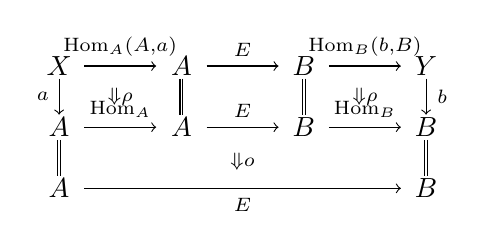
\begin{tikzpicture}[x=1.3em,y=1.3em]
  \begin{scope}[shift={(14.0,0)}]
  \node (oa1) at (0,2.6)    {$X$};
  \node (oa2) at (3.4,2.6)  {$A$};
  \node (oa3) at (6.8,2.6)  {$B$};
  \node (oa4) at (10.2,2.6) {$Y$};
  \node (oa5) at (0,0.9)    {$A$};
  \node (oa6) at (3.4,0.9)  {$A$};
  \node (oa7) at (6.8,0.9)  {$B$};
  \node (oa8) at (10.2,0.9) {$B$};
  \node (oa9) at (0,-0.8)   {$A$};
  \node (oa10) at (10.2,-0.8){$B$};
  \draw[->] (0.7,2.6) -- node[above]{$\scriptstyle\HomA(A,a)$} (2.7,2.6);
  \draw[->] (4.1,2.6) -- node[above]{$\scriptstyle E$} (6.1,2.6);
  \draw[->] (7.5,2.6) -- node[above]{$\scriptstyle\HomB(b,B)$} (9.5,2.6);
  \draw[->] (0.7,0.9) -- node[above]{$\scriptstyle\HomA$} (2.7,0.9);
  \draw[->] (4.1,0.9) -- node[above]{$\scriptstyle E$} (6.1,0.9);
  \draw[->] (7.5,0.9) -- node[above]{$\scriptstyle\HomB$} (9.5,0.9);
  \draw[->] (0.7,-0.8) -- node[below]{$\scriptstyle E$} (9.5,-0.8);
  \draw[->] (0,2.25) -- (0,1.25);
  \node at (-0.45,1.75) {$\scriptstyle a$};
  \draw[double,double distance=0.6pt] (3.4,2.25) -- (3.4,1.25);
  \draw[double,double distance=0.6pt] (6.8,2.25) -- (6.8,1.25);
  \draw[->] (10.2,2.25) -- (10.2,1.25);
  \node at (10.65,1.75) {$\scriptstyle b$};
  \node at (1.7,1.75) {$\scriptstyle\Downarrow\rho$};
  \node at (8.5,1.75) {$\scriptstyle\Downarrow\rho$};
  \draw[double,double distance=0.6pt] (0,0.55) -- (0,-0.45);
  \draw[double,double distance=0.6pt] (10.2,0.55) -- (10.2,-0.45);
  \node at (5.1,-0.05) {$\scriptstyle\Downarrow o$};
  \end{scope}
\end{tikzpicture}
\end{center}
\end{proposition}

\begin{proof}
该相容序列的水平复合\trTwoSidedFibration{}是
\begin{center}
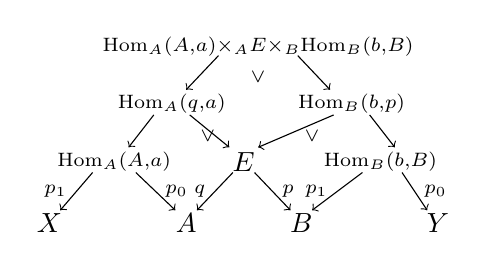
\begin{tikzpicture}[x=1.3em,y=1.3em]
  \node (pt) at (5.0,5.5)
    {$\scriptstyle\HomA(A,a)\times_{A}E\times_{B}\HomB(b,B)$};
  \node (pl) at (2.6,3.9) {$\scriptstyle\HomA(q,a)$};
  \node (pr) at (7.6,3.9) {$\scriptstyle\HomB(b,p)$};
  \draw[->] (3.9,5.25) -- (3.0,4.3);
  \draw[->] (6.1,5.25) -- (7.0,4.3);
  \node at (5.0,4.65) {$\scriptstyle\vee$};
  \node (pl1) at (1.0,2.3)  {$\scriptstyle\HomA(A,a)$};
  \node (pm) at (4.6,2.3)   {$E$};
  \node (pr1) at (8.4,2.3)  {$\scriptstyle\HomB(b,B)$};
  \draw[->] (2.1,3.6) -- (1.4,2.7);
  \draw[->] (3.1,3.6) -- (4.2,2.7);
  \node at (3.6,3.0) {$\scriptstyle\vee$};
  \draw[->] (7.1,3.6) -- (5.0,2.7);
  \draw[->] (8.1,3.6) -- (8.8,2.7);
  \node at (6.5,3.0) {$\scriptstyle\vee$};
  \node (x1) at (-0.8,0.6) {$X$};
  \node (x2) at (3.0,0.6)  {$A$};
  \node (x3) at (6.2,0.6)  {$B$};
  \node (x4) at (10.0,0.6) {$Y$};
  \draw[->] (0.4,2.0) -- node[left,pos=0.5]{$\scriptstyle p_{1}$} (-0.5,0.95);
  \draw[->] (1.6,2.0) -- node[right,pos=0.5]{$\scriptstyle p_{0}$} (2.7,0.95);
  \draw[->] (4.3,2.0) -- node[left,pos=0.5]{$\scriptstyle q$} (3.3,0.95);
  \draw[->] (4.9,2.0) -- node[right,pos=0.5]{$\scriptstyle p$} (5.9,0.95);
  \draw[->] (7.9,2.0) -- node[left,pos=0.5]{$\scriptstyle p_{1}$} (6.5,0.95);
  \draw[->] (9.0,2.0) -- node[right,pos=0.5]{$\scriptstyle p_{0}$} (9.7,0.95);
\end{tikzpicture}
\end{center}
由此我们看到，命题 8.3.11 的那个二元复合胞腔
\begin{center}
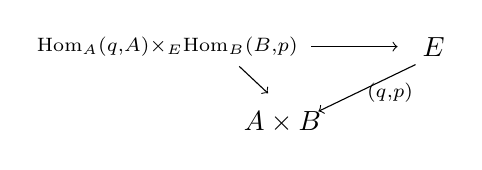
\begin{tikzpicture}[x=1.3em,y=1.3em]
  \node (bn) at (0,1.4) {$\scriptstyle\HomA(q,A)\times_{E}\HomB(B,p)$};
  \node (be) at (7.4,1.4) {$E$};
  \node (bab) at (3.2,-0.7) {$A\times B$};
  \draw[->] (4.0,1.4) -- (6.4,1.4);
  \draw[->] (2.0,0.85) -- (2.8,0.1);
  \draw[->] (6.9,0.9) -- node[right,pos=0.6]{$\scriptstyle(q,p)$} (4.2,-0.4);
\end{tikzpicture}
\end{center}
沿 $a\times b\colon X\times Y\to A\times B$ 作\trPullback，即定义出映射
$\mu$。由引理
8.3.7，我们得出结论：$\mu\colon\HomA(A,a)\divideontimes E\divideontimes\HomB(b,B)\Rightarrow E(b,a)$ 是一个强复合。

\end{proof}

当命题 8.4.7 的三元复合之源中出现的三支\trModule{}之一是单位模时，我们可以利用
引理 8.3.8 以及与该单位相关联的零元复合胞腔，把这一三元复合化归为二元复合（见%
\cref{ex:binary-strong-composites}）。这一论证证明了下面这一对推论。

\begin{corollary}\label{cor:comma-module-factors}
对函子的任意\trCospan{} $C\xrightarrow{g}A\xleftarrow{f}B$，\trCommaModule{} $\HomA(f,g)$
分解为一个强复合
\begin{center}
$\HomA(A,g)\otimes\HomA(f,A)\cong\HomA(f,g)$.
\end{center}
\end{corollary}

一个类似的化归（见练习 8.2.i）证明：右可表示模总能彼此复合，且对偶地，左可表示模
总能彼此复合：

\begin{corollary}\label{cor:represented-composites}
任何可复合的\trFunctor{}对 $A\xrightarrow{f}B\xrightarrow{g}C$ 定义一对可强复合
的右表示模与一对可强复合的左表示模
\begin{center}
$A\xrightarrow{\HomB(B,f)}B\xrightarrow{\HomC(C,g)}C$
\qquad\qquad
$C\xrightarrow{\HomC(g,C)}B\xrightarrow{\HomB(f,B)}A$
\end{center}
并且诸强复合仍是被表示的：
\begin{center}
$\HomB(B,f)\otimes\HomC(C,g)\simeq\HomC(C,gf)$，并且\\[0.3em]
$\HomC(g,C)\otimes\HomB(f,B)\simeq\HomC(gf,C)$.
\end{center}
\end{corollary}

此结果与命题 8.3.11 相结合即可证明定理 3.5.12 的一个推广，从而使我们得以检测
可表示模。

\begin{proposition}\label{prop:detect-representable-modules}
设 $A\overset{q}{\twoheadleftarrow}E\overset{p}{\twoheadrightarrow}B$ 编码一个%
\trModule{}。
\begin{enumerate}[label=(\roman*)]
\item \trModule{} $A\xrightarrow{E}B$ 是右可表示的，当且仅当其左腿
$q\colon E\twoheadrightarrow A$ 有一个\trRightAdjoint{} $r\colon A\to E$；此时
$E\simeq\HomB(B,pr)$。
\item \trModule{} $A\xrightarrow{E}B$ 是左可表示的，当且仅当其右腿
$p\colon E\twoheadrightarrow B$ 有一个\trLeftAdjoint{} $\ell\colon B\to E$；此时
$E\simeq\HomA(q\ell,A)$。
\end{enumerate}
\end{proposition}

\begin{proof}
由引理 3.5.9 与定理 3.5.12，所论的诸伴随与诸\trFiberedEquivalence{}对可表示模
而言存在，故只需证明其逆命题。
由命题 8.3.11，任何\trModule{} $E$ 都可以表达为复合
$\HomA(q,A)\otimes\HomB(B,p)\simeq E$，即其左腿的左表示后接其右腿的右表示。
若 $q\dashv r$，则由命题 4.1.1，$\HomA(q,A)\simeq\HomE(E,r)$（作为从 $A$ 到 $E$
的\trModule）；于是由引理 8.3.3，
$\HomE(E,r)\otimes\HomB(B,p)\simeq E$。
由\cref{cor:represented-composites}，
$\HomE(E,r)\otimes\HomB(B,p)\simeq\HomB(B,pr)$，故再由引理 8.3.3 一次，即得
$\HomB(B,pr)\simeq E$。
\end{proof}

最后，我们重新审视推论 3.5.11 中给出的\trYonedaLemma{}的「廉价」版本，它把%
\trHomotopyTwoCategory{}中的\trNaturalTransformation{}编码为诸表示模的映射。

\begin{proposition}\label{prop:two-cell-bijections}
对任何平行\trFunctor{}对，\trHomotopyTwoCategory{}中的 2-胞腔
\begin{center}
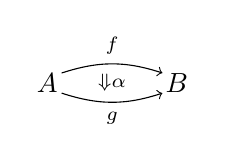
\begin{tikzpicture}[x=1.3em,y=1.3em]
  \node (pa) at (0,0) {$A$};
  \node (pb) at (3.6,0) {$B$};
  \draw[->] (0.4,0.28) to[bend left=18] node[above,pos=0.5]{$\scriptstyle f$} (3.2,0.28);
  \draw[->] (0.4,-0.28) to[bend right=18] node[below,pos=0.5]{$\scriptstyle g$} (3.2,-0.28);
  \node at (1.8,0) {$\scriptstyle\Downarrow\alpha$};
\end{tikzpicture}
\end{center}
与模的\trVirtualEquipment{}中的诸胞腔之间存在自然双射：
\begin{center}
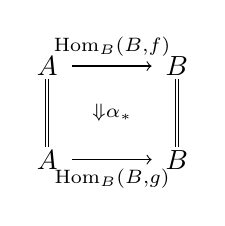
\begin{tikzpicture}[x=1.3em,y=1.3em]
  \node (qa1) at (0,1.4)  {$A$};
  \node (qa2) at (3.6,1.4){$B$};
  \node (qa3) at (0,-1.2) {$A$};
  \node (qa4) at (3.6,-1.2){$B$};
  \draw[->] (0.7,1.4) -- node[above]{$\scriptstyle\HomB(B,f)$} (2.9,1.4);
  \draw[->] (0.7,-1.2) -- node[below]{$\scriptstyle\HomB(B,g)$} (2.9,-1.2);
  \draw[double,double distance=0.6pt] (0,1.05) -- (0,-0.85);
  \draw[double,double distance=0.6pt] (3.6,1.05) -- (3.6,-0.85);
  \node at (1.8,0.1) {$\scriptstyle\Downarrow\alpha_{*}$};
\end{tikzpicture}
\qquad $\mathrel{\leftrightsquigarrow}$ \qquad
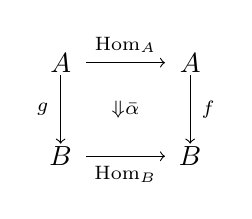
\begin{tikzpicture}[x=1.3em,y=1.3em]
  \begin{scope}[shift={(7.6,0)}]
  \node (qb1) at (0,1.4)  {$A$};
  \node (qb2) at (3.6,1.4){$A$};
  \node (qb3) at (0,-1.2) {$B$};
  \node (qb4) at (3.6,-1.2){$B$};
  \draw[->] (0.7,1.4) -- node[above]{$\scriptstyle\HomA$} (2.9,1.4);
  \draw[->] (0.7,-1.2) -- node[below]{$\scriptstyle\HomB$} (2.9,-1.2);
  \draw[->] (0,1.05) -- (0,-0.85);
  \node at (-0.5,0.1) {$\scriptstyle g$};
  \draw[->] (3.6,1.05) -- (3.6,-0.85);
  \node at (4.1,0.1) {$\scriptstyle f$};
  \node at (1.8,0.1) {$\scriptstyle\Downarrow\bar{\alpha}$};
  \end{scope}
\end{tikzpicture}
\qquad $\mathrel{\leftrightsquigarrow}$ \qquad
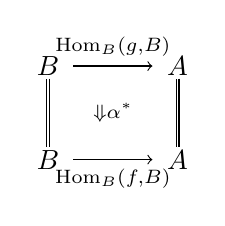
\begin{tikzpicture}[x=1.3em,y=1.3em]
  \begin{scope}[shift={(15.2,0)}]
  \node (qc1) at (0,1.4)  {$B$};
  \node (qc2) at (3.6,1.4){$A$};
  \node (qc3) at (0,-1.2) {$B$};
  \node (qc4) at (3.6,-1.2){$A$};
  \draw[->] (0.7,1.4) -- node[above]{$\scriptstyle\HomB(g,B)$} (2.9,1.4);
  \draw[->] (0.7,-1.2) -- node[below]{$\scriptstyle\HomB(f,B)$} (2.9,-1.2);
  \draw[double,double distance=0.6pt] (0,1.05) -- (0,-0.85);
  \draw[double,double distance=0.6pt] (3.6,1.05) -- (3.6,-0.85);
  \node at (1.8,0.1) {$\scriptstyle\Downarrow\alpha^{*}$};
  \end{scope}
\end{tikzpicture}
\end{center}
\end{proposition}

\begin{proof}
$\Mod(\mathcal{K})$ 中的诸双射随后可以由\cref{thm:spider-lemma}与%
\cref{cor:compatible-sequence-bijection} 导出。\trHomotopyTwoCategory{}中的
2-胞腔与左、右可表示元之间的一元模映射之间的那个双射，不过是推论 3.5.11 的一个
复述。
\end{proof}

\begin{definition}[协变嵌入与逆变嵌入]%
\label{def:covariant-contravariant-embeddings}
\cref{prop:two-cell-bijections} 定义了两个在对象上恒同的\trLocallyFullyFaithful{}%
\trHomomorphism{}在 2-胞腔上的作用
\begin{center}
$\mathfrak{h}\mathcal{K}\hooklongrightarrow\Mod(\mathcal{K})$
\qquad\qquad
$\mathfrak{h}\mathcal{K}^{\mathrm{coop}}\hooklongrightarrow\Mod(\mathcal{K})$
\\[0.6em]
$A\xrightarrow{f}B\longmapsto A\xrightarrow{\HomB(B,f)}B$
\qquad\qquad
$A\xrightarrow{f}B\longmapsto B\xrightarrow{\HomB(f,B)}A$
\end{center}
它们给出\trHomotopyTwoCategory{}到 $\Mod(\mathcal{K})$ 的那个只含竖直边界皆为
恒同的一元胞腔的子「\trBicategory」的\trFullyFaithful{}嵌入。
$\Mod(\mathcal{K})$ 的这一子结构尚不是一个\trBicategory，因为并非所有水平可复合的%
\trModule{}都可复合；但若只限制到诸右可表示模、或只限制到诸左可表示模，则由%
\cref{cor:represented-composites}，诸复合确实存在，且这两个嵌入定义出真正的二
范畴\trHomomorphism：给定 $A\xrightarrow{f}B\xrightarrow{g}C$，我们有
$\HomB(B,f)\otimes\HomC(C,g)\simeq\HomC(C,gf)$ 与
$\HomC(g,C)\otimes\HomB(f,B)\simeq\HomC(gf,C)$。我们分别把它们称作%
\textbf{协变嵌入}（covariant embedding）与\textbf{逆变嵌入}（contravariant
embedding）。
\end{definition}

\begin{remark}\label{rem:third-embedding}
除协变嵌入与逆变嵌入之外，还有第三种把\trHomotopyTwoCategory{}
$\mathfrak{h}\mathcal{K}$ 嵌入 $\Mod(\mathcal{K})$ 的\trLocallyFullyFaithful{}嵌入：
它在对象上
为恒同，把 $f\colon A\to B$ 送到相应的竖直 1-胞腔，并利用%
\cref{prop:two-cell-bijections}的第三个双射来定义其在 2-胞腔上的作用。由于
$\HomA\otimes\HomA\simeq\HomA$，该嵌入的像中的一元胞腔既可以水平复合又可以竖直
复合，而且这个嵌入在两个方向上都是函子性的：$\mathfrak{h}\mathcal{K}$ 中%
\trNaturalTransformation{}的竖直复合与一元胞腔的水平复合相重合，而
$\mathfrak{h}\mathcal{K}$ 中\trNaturalTransformation{}的水平复合与一元胞腔的
竖直复合相重合。这个像恰好是命题 8.3.18 的竖直 2-范畴。然而，我们对定义 8.4.12
的协变嵌入与逆变嵌入的使用要多得多。
\end{remark}

\subsection*{练习}

\begin{exercise}\label{ex:companion-conjoint-any-equipment}
在任意\trVirtualEquipment{}中证明\cref{prop:representable-restriction-application}，
而不诉诸引理 8.1.16。
\end{exercise}

\begin{exercise}\label{ex:spider-generalization}
请陈述并证明\cref{thm:spider-lemma}的一个推广，其中陈述中出现的底部那个
$n+2$ 元胞腔并非纤维化映射，其竖直边界由任意一对非恒同的\trFunctor{}给出。
\end{exercise}

\begin{exercise}\label{ex:binary-strong-composites}
请证明\cref{prop:ternary-strong-composite}的一个二元版本：对任意\trModule{}
$A\xrightarrow{E}B$ 与任意\trFunctor{} $a\colon X\to A$、$b\colon Y\to B$，强复合
$\HomA(A,a)\otimes E$ 与 $E\otimes\HomB(b,B)$ 存在，且分别由限制 $E(1,a)$ 与
$E(b,1)$ 给出。
\end{exercise}

\begin{exercise}\label{ex:nonstrong-ternary}
请在任意\trVirtualEquipment{}中证明\cref{prop:ternary-strong-composite}的非强
版本，而不诉诸引理 8.3.7。
\end{exercise}

\begin{exercise}\label{ex:adjoint-representables}
对任意\trFunctor{} $f\colon A\to B$，请定义一个\trCanonical{}一元胞腔
$\eta\colon\HomA\Rightarrow\HomB(f,f)\simeq\HomB(B,f)\otimes\HomB(f,B)$ 与一个
二元胞腔
$\epsilon\colon\HomB(f,B)\times\HomB(B,f)\Rightarrow\HomB$。请利用这些数据证明：
诸\trModule{} $A\xrightarrow{\HomB(B,f)}B$ 与
$B\xrightarrow{\HomB(f,B)}A$ 在某种适宜的意义下是「伴随的」。
\end{exercise}

